\documentclass[12pt, a4paper]{article}
\usepackage[utf8]{inputenc}
\usepackage[T1]{fontenc}
\usepackage{geometry}
\geometry{margin=1in, top=1.2in, bottom=1.1in, left=1.25in, right=1.25in, footskip=40pt}
\usepackage{mathptmx}           % Times New Roman for text and math
\usepackage{setspace}
\doublespacing
\usepackage{graphicx}
\usepackage{caption}
\captionsetup[figure]{labelfont=bf, textfont=it, labelsep=period}
\captionsetup[table]{labelfont=bf, textfont=it, labelsep=period, position=top}
\usepackage{xcolor}
\usepackage{hyperref}
\hypersetup{colorlinks=true, linkcolor=black, citecolor=black, urlcolor=blue}
\usepackage{apacite}
\usepackage{tikz}
\usetikzlibrary{shapes.geometric, arrows.meta, positioning, calc}
\usepackage{amsmath}
\usepackage{amssymb}
\usepackage{booktabs}
\usepackage{multirow}
\usepackage{fancyhdr}
\usepackage{titlesec}
\usepackage{enumitem}
\usepackage{microtype}
\usepackage{afterpage}

% ---- Section heading formats (match JISE: unnumbered, centred, all-caps, bold) ----
\setcounter{secnumdepth}{0}
\titleformat{\section}
  {\normalfont\normalsize\bfseries\centering}
  {}{0em}{\MakeUppercase}
\titlespacing{\section}{0pt}{18pt plus 4pt minus 2pt}{6pt plus 2pt}

\titleformat{\subsection}
  {\normalfont\normalsize\bfseries}
  {}{0em}{}
\titlespacing{\subsection}{0pt}{12pt plus 2pt minus 2pt}{4pt plus 1pt}

\titleformat{\subsubsection}
  {\normalfont\normalsize\itshape}
  {}{0em}{}
\titlespacing{\subsubsection}{0pt}{8pt}{3pt}

% ---- Headers and footers ----
\pagestyle{fancy}
\fancyhf{}
\renewcommand{\headrulewidth}{0pt}
\renewcommand{\footrulewidth}{0pt}
% Page 1: page number at bottom centre only
\fancypagestyle{firstpage}{
    \fancyhf{}
    \fancyfoot[C]{\thepage}
}
% Page 2 onward copyright footer (compact single line)
\fancypagestyle{secondpage}{
    \fancyhf{}
    \fancyhead[L]{\footnotesize\itshape Journal of Interdisciplinary Studies in Education}
    \fancyhead[R]{\footnotesize\itshape Gudekar \& Nanade}
    \renewcommand{\headrulewidth}{0.4pt}
    \fancyfoot[C]{\thepage}
}
% Inner pages: running heads + page number
\fancypagestyle{innerpages}{
    \fancyhf{}
    \fancyhead[L]{\footnotesize\itshape Journal of Interdisciplinary Studies in Education}
    \fancyhead[R]{\footnotesize\itshape Gudekar \& Nanade}
    \renewcommand{\headrulewidth}{0.4pt}
    \fancyfoot[C]{\thepage}
}

\begin{document}
\thispagestyle{firstpage}

\noindent\textbf{Article}\hfill
\begin{minipage}[t]{0.72\linewidth}
  \raggedleft\small
  \textcolor{blue!70!black}{\textbf{Journal of Interdisciplinary Studies in Education}}\\
  Volume XX, Issue X (202X), pp.\ XX--XX\\
  \textit{Journal of Interdisciplinary Studies in Education}\\
  ISSN: 2166-2681 Print\ 2690-0408 Online $|$ \url{https://ojed.org/jise}\\
  \url{https://doi.org/10.32674/XXXXX}
\end{minipage}

\noindent\rule{\textwidth}{0.5pt}

\vspace{1.2em}

\begin{center}
{\large\bfseries Multiple Intelligences as Predictors of RIASEC Vocational Domains:\\[3pt]
A Machine Learning and Explainable AI Framework for\\[3pt]
Psychometric Career Counseling}
\end{center}

\vspace{0.6em}

\begin{center}
Sanket Gudekar\\
\textit{Mukesh Patel School of Technology Management \& Engineering, SVKM's NMIMS, Mumbai, India}\\[5pt]
Sunny Nanade$^{*}$\\
\textit{Mukesh Patel School of Technology Management \& Engineering, SVKM's NMIMS, Mumbai, India}\\
ORCID: 0000-0001-7098-1084\\
{\small $^{*}$Corresponding Author: \href{mailto:sunny.nanade@nmims.edu}{sunny.nanade@nmims.edu}}
\end{center}

\vspace{0.6em}
\noindent\rule{\textwidth}{0.4pt}
\vspace{0.3em}

\begin{center}
\textbf{ABSTRACT}
\end{center}

\begin{singlespacing}
\noindent This study empirically investigates the predictive relationship between Howard Gardner's Multiple Intelligences (MI) and John Holland's RIASEC vocational framework using machine learning. Psychometric assessment data from 107 high school students (Mumbai, India) were extracted via a dual-parser automated PDF pipeline and rigorously verified against the psychometric instrument's scoring formulae. Four classifiers were evaluated under stratified five-fold cross-validation. Logistic regression achieved the highest cross-validated accuracy of 81.5\%, substantially outperforming both the majority-class baseline (30.8\%) and the equal-probability random baseline (16.7\%), with a one-sample $t$-test against the null confirming statistical significance ($t(4) = 14.48$, $p < .001$). The hold-out accuracy on an independent test set ($n = 27$) was 88.9\%. Unsupervised K-Means clustering on PCA-projected MI profiles identified three cognitive engagement archetypes (\textit{High}, \textit{Moderate}, \textit{Developing}). SHAP-based explainable AI, applied to the Random Forest model, revealed that Naturalist, Bodily-Kinesthetic, and Interpersonal intelligences collectively drive RIASEC domain differentiation. Empirical verification of all six RIASEC scoring formulae further revealed that Verbal-Linguistic and Musical intelligences are structurally absent from all vocational domain scores. These findings provide empirical and computationally transparent evidence that MI profiles reliably predict dominant RIASEC domains, supporting their integration into data-driven psychometric career counseling systems.
\end{singlespacing}

\vspace{0.4em}
\noindent\textit{\textbf{Keywords:}} multiple intelligences, RIASEC, Holland's vocational model, machine learning, career counseling, explainable AI, SHAP, psychometric assessment, educational data mining
\vspace{0.2em}
\noindent\rule{\textwidth}{0.4pt}

\vspace{0.5cm}

\section{Introduction}
\pagestyle{secondpage}

{\footnotesize\singlespacing\noindent
\textcopyright~Author(s), 2026. Published by Star Scholars Press. This article is distributed under the Creative Commons Attribution 4.0 International License (CC BY 4.0), which permits unrestricted use, distribution, and reproduction in any medium, provided that the original author and source are credited. \url{https://creativecommons.org/licenses/by/4.0/}}

\bigskip

Career choice is among the most consequential decisions in a student's educational trajectory, yet many students navigate this process without systematic assessment of their cognitive strengths and vocational inclinations \cite{leung2022new}. Traditional career counselling has relied mainly on the subjective expertise of counsellors and the use of static psychometric tools, thus creating a need for more objective, scalable, and data-driven approaches \cite{elhaji2020proposal}.

Two major theoretical frameworks have served as the foundations of modern vocational assessment. Multiple Intelligences (MI) is a theory developed by Howard Gardner that suggests human cognition comprises eight distinct modalities: Verbal-Linguistic, Logical-Mathematical, Spatial-Visual, Bodily-Kinesthetic, Musical, Interpersonal, Intrapersonal, and Naturalist \cite{gardner2011frames}. There is neuroscientific evidence to support this pluralistic view of cognition \cite{shearer2018multiple}. At the same time, the RIASEC model by John Holland classifies vocational personalities into six domains: Realistic, Investigative, Artistic, Social, Enterprising, and Conventional \cite{holland1997making}. Holland's hexagonal model remains the most widely adopted framework in career counselling worldwide \cite{nauta2010holland}.

While both frameworks are theoretically complementary---each characterizing individuals along multidimensional psychological constructs---few previous studies have used modern computational methods to explore the predictive relationship between them. Most existing computer-assisted career guidance systems (CACGS) rely on static rule-based mappings or simple statistical correlations \cite{leung2022new}. Machine learning (ML) offers a methodological advance, revealing non-linear and interactive predictive relationships that conventional statistical methods may fail to identify \cite{romero2020educational}. Earlier work by Kamal et al. \citeyear{kamal2021smart} demonstrated a career guidance system employing both MI and RIASEC through ML classifiers, while a recent meta-analysis by Song et al. \citeyear{song2024investigating} quantified the advantage of ML over traditional statistical models in career choice prediction. However, these systems have typically treated MI and RIASEC as independent input sources rather than examining the structural mathematical relationship between them.

Artificial intelligence (AI) has been growing in importance in higher education and student assessment, as documented in recent systematic reviews \cite{crompton2023artificial, zawacki2019systematic, chen2020artificial}. Predictive analytics and early warning systems have empirically demonstrated a positive impact on student counseling outcomes \cite{plak2021early}. Of particular relevance, Guleria and Sood \citeyear{guleria2022explainable} showed that explainable AI (XAI) classifiers work well for educational data mining in career counselling, highlighting the critical importance of model transparency for educator trust and adoption.

Building upon prior frameworks for ML-based continuous student learning assessment \cite{nanade2021predictive, nanade2020model}, this study investigates the following research questions:
\begin{enumerate}
    \item Can a student's dominant RIASEC vocational domain be accurately predicted from their eight MI scores using machine learning classifiers?
    \item Which specific MI dimensions are the strongest predictors of vocational aptitude, and can this be made transparent through explainable AI?
    \item Do students naturally cluster into distinct cognitive archetypes based on their MI profiles?
\end{enumerate}

The primary contribution of this study is an empirical, end-to-end pipeline that transitions psychometric evaluation from descriptive observation to predictive science, while maintaining full model transparency through SHapley Additive exPlanations (SHAP) \cite{lundberg2017unified}.

\section{Literature Review}

\subsection{Gardner's Theory of Multiple Intelligences}

In his groundbreaking work, Gardner \citeyear{gardner2011frames} argued that intelligence is not a single construct measurable by an IQ score, but rather a collection of relatively independent cognitive capacities. The theory identifies eight intelligences, each linked to distinct brain regions and developmental trajectories: Linguistic, Logical-Mathematical, Spatial, Bodily-Kinesthetic, Musical, Interpersonal, Intrapersonal, and Naturalist. Since its introduction, MI theory has been widely applied in educational practice for curriculum design, student assessment, and personalized instruction \cite{shearer2018multiple}. Psychometric instruments based on MI theory typically employ Likert-scale self-report questionnaires that yield a profile of relative cognitive strengths across the eight domains.

\subsection{Holland's RIASEC Model}

Holland's \citeyear{holland1997making} theory of vocational personalities states that individuals can be described by their similarity to six personality types---Realistic, Investigative, Artistic, Social, Enterprising, and Conventional---and that career satisfaction and stability are best achieved when personality type matches the work environment. The RIASEC model has been widely validated across cultures, age groups, and occupational settings \cite{nauta2010holland}. The field of vocational psychology has developed significantly in parallel with advances in psychometric methodology \cite{sackett2017individualized}.

\subsection{Machine Learning in Educational Data Mining}

The use of ML in educational data has increased significantly, with systematic reviews identifying prediction, classification, and clustering as the three main analytical tasks \cite{romero2020educational, zawacki2019systematic}. Random forests \cite{breiman2001random}, logistic regression, and support vector machines are among the most commonly used algorithms in student performance prediction and career recommendation systems \cite{guleria2022explainable}. Chen et al. \citeyear{chen2020artificial} comprehensively reviewed AI in education, highlighting the importance of models that are both accurate and interpretable. The TRIPOD+AI guidelines \cite{collins2024tripod} have also established formal reporting standards for prediction models that use ML methods.

Most pertinent to the present study, Kamal et al. \citeyear{kamal2021smart} designed a smart career guidance system using both Gardner's MI framework and Holland's RIASEC model with machine learning classifiers, demonstrating the feasibility of combining MI and RIASEC in computational guidance systems. A recent large-scale meta-analysis by Song et al. \citeyear{song2024investigating} quantified ML's advantage in career choice prediction across multiple studies, establishing that ML classifiers consistently outperform traditional statistical approaches---findings that contextualize the strong logistic regression performance observed in the present study.

\subsection{Explainable AI in Education}

One of the central challenges in applying ML in educational contexts is the ``black box'' problem---complex models may perform well but provide no understanding of how they reach their decisions. Grounded in cooperative game theory, the SHAP framework provides a principled method for computing the marginal contribution of each feature to individual predictions \cite{lundberg2017unified}. Guleria and Sood \citeyear{guleria2022explainable} demonstrated that XAI techniques are essential for career counseling applications, as human counselors must understand and validate algorithmic recommendations before acting on them. Zahour et al. \citeyear{zahour2019automatic} further showed that interpretable multi-class neural network classifiers can effectively align academic and vocational guidance questions with theoretical career frameworks, underscoring the importance of model transparency in educational advisory systems. AI literacy and ethical transparency have been recognized as priorities for responsible deployment in educational systems \cite{zhang2022integrating}.

\section{Methodology}

\subsection{Data Collection and Ethical Considerations}

The data consisted of 107 psychometric assessment reports of high school students. All reports were produced by a standardized, commercially administered 80-item Multiple Intelligences test instrument. Reports were submitted in PDF format and included structured MI scores, domain scores, RIASEC vocational scores, and career probability estimates. All personally identifiable information (PII)---including names, dates of birth, email addresses, and contact numbers---was removed during the data extraction process to ensure student privacy. Informed consent was obtained from participants for use of their anonymized psychometric data in research.

\subsection{Psychometric Instrument}

This questionnaire consisted of 80 items assessing the eight MI modalities (10 items per intelligence). Each statement was rated on a 4-point Likert scale (1 = Mostly Disagree, 2 = Slightly Disagree, 3 = Slightly Agree, 4 = Mostly Agree), yielding raw scores in the range [10, 40] per intelligence.

Three macro-domain scores were calculated as percentages of the total MI score:
\begin{equation}
\text{Analytical}(\%) = \frac{\text{LM} + \text{Mus} + \text{Nat}}{\sum_{i=1}^{8} MI_i} \times 100
\end{equation}
\begin{equation}
\text{Interactive}(\%) = \frac{\text{VL} + \text{Inter} + \text{BK}}{\sum_{i=1}^{8} MI_i} \times 100
\end{equation}
\begin{equation}
\text{Introspective}(\%) = \frac{\text{Intra} + \text{SV}}{\sum_{i=1}^{8} MI_i} \times 100
\end{equation}

RIASEC scores were derived from weighted combinations of MI raw scores, each normalized to a 0--10 scale by dividing by the theoretical maximum of the constituent raw scores (each bounded in [10, 40]). The formulas were empirically verified by recomputing each student's RIASEC scores from their raw MI data (maximum re-derivation error $< 0.01$ across all 107 records):
\begin{equation}
R = \frac{\text{BK} + \text{Nat}}{80} \times 10, \quad
S = \frac{\text{Nat} + \text{Inter}}{80} \times 10, \quad
C = \frac{\text{Intra} + \text{LM}}{80} \times 10
\end{equation}
\begin{equation}
I = \frac{\text{BK} + \text{Intra} + \text{LM} + \text{SV}}{160} \times 10, \quad
A = \frac{\text{SV} + \text{Intra} + \text{Nat}}{120} \times 10, \quad
E = \frac{\text{BK} + \text{LM} + \text{Inter}}{120} \times 10
\end{equation}

The denominators are the theoretical maximum sum of the constituents (two MIs: max $= 2 \times 40 = 80$; three MIs: max $= 3 \times 40 = 120$; four MIs: max $= 4 \times 40 = 160$), ensuring all RIASEC scores are bounded within $[0, 10]$. Table~\ref{tab:formula_membership} summarises which MI dimensions contribute to each RIASEC domain.

\begin{table}[htpb]
\centering
\caption{MI Component Membership in RIASEC Formulas}
\label{tab:formula_membership}
\small
\begin{tabular}{lccccccc}
\toprule
MI Dimension & R & I & A & S & E & C & Count \\
\midrule
Verbal-Linguistic (VL)    & -- & -- & -- & -- & -- & -- & 0 \\
Logical-Mathematical (LM) & -- & \checkmark & -- & -- & \checkmark & \checkmark & 3 \\
Spatial-Visual (SV)       & -- & \checkmark & \checkmark & -- & -- & -- & 2 \\
Bodily-Kinesthetic (BK)   & \checkmark & \checkmark & -- & -- & \checkmark & -- & 3 \\
Musical (Mus)             & -- & -- & -- & -- & -- & -- & 0 \\
Interpersonal (Inter)     & -- & -- & -- & \checkmark & \checkmark & -- & 2 \\
Intrapersonal (Intra)     & -- & \checkmark & \checkmark & -- & -- & \checkmark & 3 \\
Naturalist (Nat)          & \checkmark & -- & \checkmark & \checkmark & -- & -- & 3 \\
\bottomrule
\end{tabular}
\end{table}

Notably, Verbal-Linguistic and Musical intelligences do not feature in any RIASEC formula, indicating that they represent cognitive capacities orthogonal to the vocational personality dimensions captured by Holland's hexagonal model.

\subsection{Automated Data Extraction and Verification}

A robust automated extraction pipeline was developed to eliminate human transcription errors and ensure complete data integrity. Two independent parsers were implemented: a text-based regex parser using \texttt{pdfplumber} and a spatial coordinate parser using \texttt{PyMuPDF}. Both parsers extracted MI raw scores, percentages, ranks, domain scores, and RIASEC scores from each PDF report.

After extraction, rigorous statistical verification was performed. Unit tests confirmed: (a) all MI raw scores fell within the valid [10, 40] range; (b) all RIASEC scores were bounded within [0, 10]; (c) no constant or duplicated columns existed; and (d) the RIASEC scores could be independently re-derived from the raw MI scores using the verified formulas (Equations 4--5), with all re-derived scores matching within rounding tolerance ($< 0.01$) for all 107 records. Median imputation was applied to the small number of career probability fields that could not be extracted due to PDF parsing inconsistencies; all MI raw scores and RIASEC scores were complete for every record.

Figure~\ref{fig:flowchart} illustrates the complete computational pipeline.

\begin{figure}[htpb]
\centering
\resizebox{\textwidth}{!}{
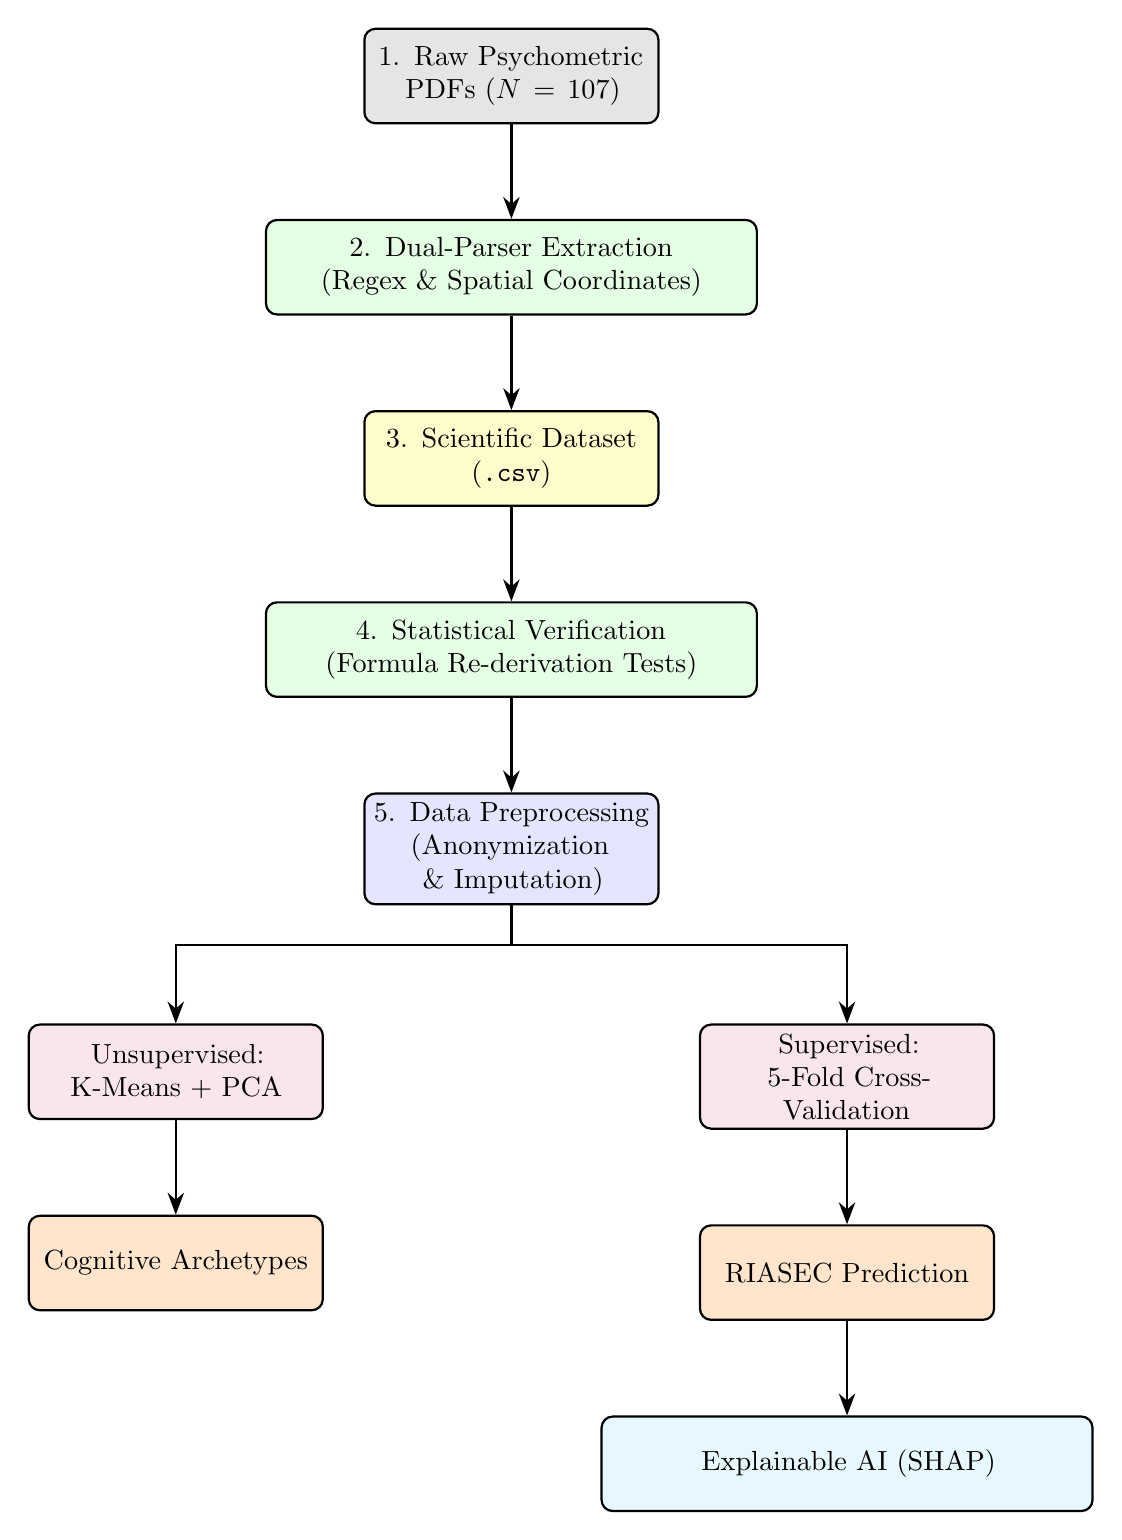
\begin{tikzpicture}[
    node distance=1.2cm and 1cm,
    box/.style={rectangle, draw=black, thick, fill=blue!10, text width=3.5cm, align=center, rounded corners, minimum height=1.2cm},
    widebox/.style={rectangle, draw=black, thick, fill=green!10, text width=6cm, align=center, rounded corners, minimum height=1.2cm},
    arrow/.style={-{Stealth[scale=1.2]}, thick, draw=black}
]
    \node (raw) [box, fill=gray!20] {1. Raw Psychometric PDFs ($N=107$)};
    \node (extract) [widebox, below=of raw] {2. Dual-Parser Extraction\\(Regex \& Spatial Coordinates)};
    \node (data) [box, fill=yellow!20, below=of extract] {3. Scientific Dataset\\(\texttt{.csv})};
    \node (verify) [widebox, below=of data] {4. Statistical Verification\\(Formula Re-derivation Tests)};
    \node (preproc) [box, below=of verify] {5. Data Preprocessing\\(Anonymization \& Imputation)};

    \node (unsuper) [box, fill=purple!10, below left=1.5cm and 0.5cm of preproc] {Unsupervised:\\K-Means + PCA};
    \node (arch) [box, fill=orange!20, below=of unsuper] {Cognitive Archetypes};

    \node (super) [box, fill=purple!10, below right=1.5cm and 0.5cm of preproc] {Supervised:\\5-Fold Cross-Validation};
    \node (pred) [box, fill=orange!20, below=of super] {RIASEC Prediction};
    \node (xai) [widebox, fill=cyan!10, below=of pred] {Explainable AI (SHAP)};

    \draw [arrow] (raw) -- (extract);
    \draw [arrow] (extract) -- (data);
    \draw [arrow] (data) -- (verify);
    \draw [arrow] (verify) -- (preproc);
    \draw [arrow] (preproc.south) -- ++(0,-0.5) -| (unsuper.north);
    \draw [arrow] (preproc.south) -- ++(0,-0.5) -| (super.north);
    \draw [arrow] (unsuper) -- (arch);
    \draw [arrow] (super) -- (pred);
    \draw [arrow] (pred) -- (xai);
\end{tikzpicture}
}
\caption{Computational pipeline from raw PDF extraction through unsupervised clustering and supervised predictive classification with explainable AI.}
\label{fig:flowchart}
\end{figure}

\subsection{Unsupervised Learning: Cognitive Archetypes}

The eight MI features were standardized using $z$-score normalization and projected onto two dimensions using Principal Component Analysis (PCA) to explore inherent groupings in the student population. K-Means clustering was then applied, with the number of clusters determined by the Elbow method and validated using the Silhouette Score.

\subsection{Supervised Learning: Predictive Classification}

The classification problem was formulated as a six-class prediction problem, where the target variable $Y$ was defined as each student's highest-scoring RIASEC domain. The eight MI raw scores served as the feature vector $\mathbf{X} \in \mathbb{R}^{8}$.

Four classifiers were rigorously evaluated:
\begin{enumerate}
    \item \textbf{Logistic Regression} (multinomial, max iterations = 1000)
    \item \textbf{Support Vector Machine} (RBF kernel)
    \item \textbf{Random Forest} ($n=100$ trees, max depth = 5) \cite{breiman2001random}
    \item \textbf{Gradient Boosting} ($n=100$ estimators, max depth = 3)
\end{enumerate}

All models were evaluated using stratified 5-fold cross-validation to produce robust accuracy estimates on the small dataset ($N = 107$). For Logistic Regression and SVM, features were standardized using $z$-score normalization. All implementations used Scikit-learn \cite{pedregosa2011scikit}.

\subsection{Explainable AI via SHAP}

To satisfy the ethical requirement of transparency in educational AI \cite{guleria2022explainable}, SHapley Additive exPlanations (SHAP) were computed using a TreeExplainer \cite{lundberg2017unified}. SHAP values are both globally and locally interpretable, quantifying the marginal contribution of each MI score to the prediction for each RIASEC class.

\section{Results}

\subsection{Descriptive Statistics}

Descriptive statistics for each of the eight MI raw scores are provided in Table~\ref{tab:mi_stats}. The scores showed adequate variability across the sample, with means ranging from 28.64 (Naturalist) to 32.11 (Bodily-Kinesthetic). All distributions had low skewness ($|skew| < 0.80$) and were thus approximately normal, suitable for parametric analysis.

\begin{table}[htpb]
\centering
\caption{Descriptive Statistics for Multiple Intelligence Raw Scores ($N = 107$)}
\label{tab:mi_stats}
\small
\begin{tabular}{lcccccc}
\toprule
Intelligence & $M$ & $SD$ & Min & Max & Skew & Kurt \\
\midrule
Verbal-Linguistic     & 28.95 & 3.99 & 21 & 37 & 0.12  & $-0.86$ \\
Logical-Mathematical  & 29.39 & 3.98 & 15 & 37 & $-0.79$ & 1.09 \\
Spatial-Visual        & 30.38 & 4.06 & 20 & 39 & $-0.17$ & 0.14 \\
Bodily-Kinesthetic    & 32.11 & 3.69 & 20 & 39 & $-0.66$ & 0.64 \\
Musical               & 30.33 & 5.45 & 15 & 40 & $-0.28$ & $-0.36$ \\
Interpersonal         & 32.00 & 4.36 & 22 & 40 & $-0.49$ & $-0.15$ \\
Intrapersonal         & 30.38 & 3.87 & 21 & 40 & 0.01  & $-0.32$ \\
Naturalist            & 28.64 & 5.04 & 17 & 38 & $-0.24$ & $-0.75$ \\
\bottomrule
\end{tabular}
\end{table}

The distribution of dominant RIASEC types was imbalanced: Enterprising ($n = 33$, 30.8\%), Realistic ($n = 24$, 22.4\%), Conventional ($n = 20$, 18.7\%), Social ($n = 13$, 12.1\%), Investigative ($n = 9$, 8.4\%), and Artistic ($n = 8$, 7.5\%). This class imbalance reflects the natural distribution of vocational preferences in the student sample and is accounted for through stratified cross-validation.

The Pearson correlation matrix of MI raw scores and RIASEC domain scores is presented in Figure~\ref{fig:mi_riasec_corr}. The pattern of high correlations directly mirrors the formula membership structure (Table~\ref{tab:formula_membership}): Naturalist shows the highest correlations with Realistic ($r = .89$), Artistic ($r = .85$), and Social ($r = .84$); Logical-Mathematical correlates highest with Conventional ($r = .86$) and Investigative ($r = .73$); and Verbal-Linguistic and Musical---absent from all RIASEC formulas---show uniformly lower correlations ($r = .32$--.55), consistent with their formula-independent status. This pattern provides strong empirical validation of the psychometric instrument's scoring structure.

\begin{figure}[htpb]
    \centering
    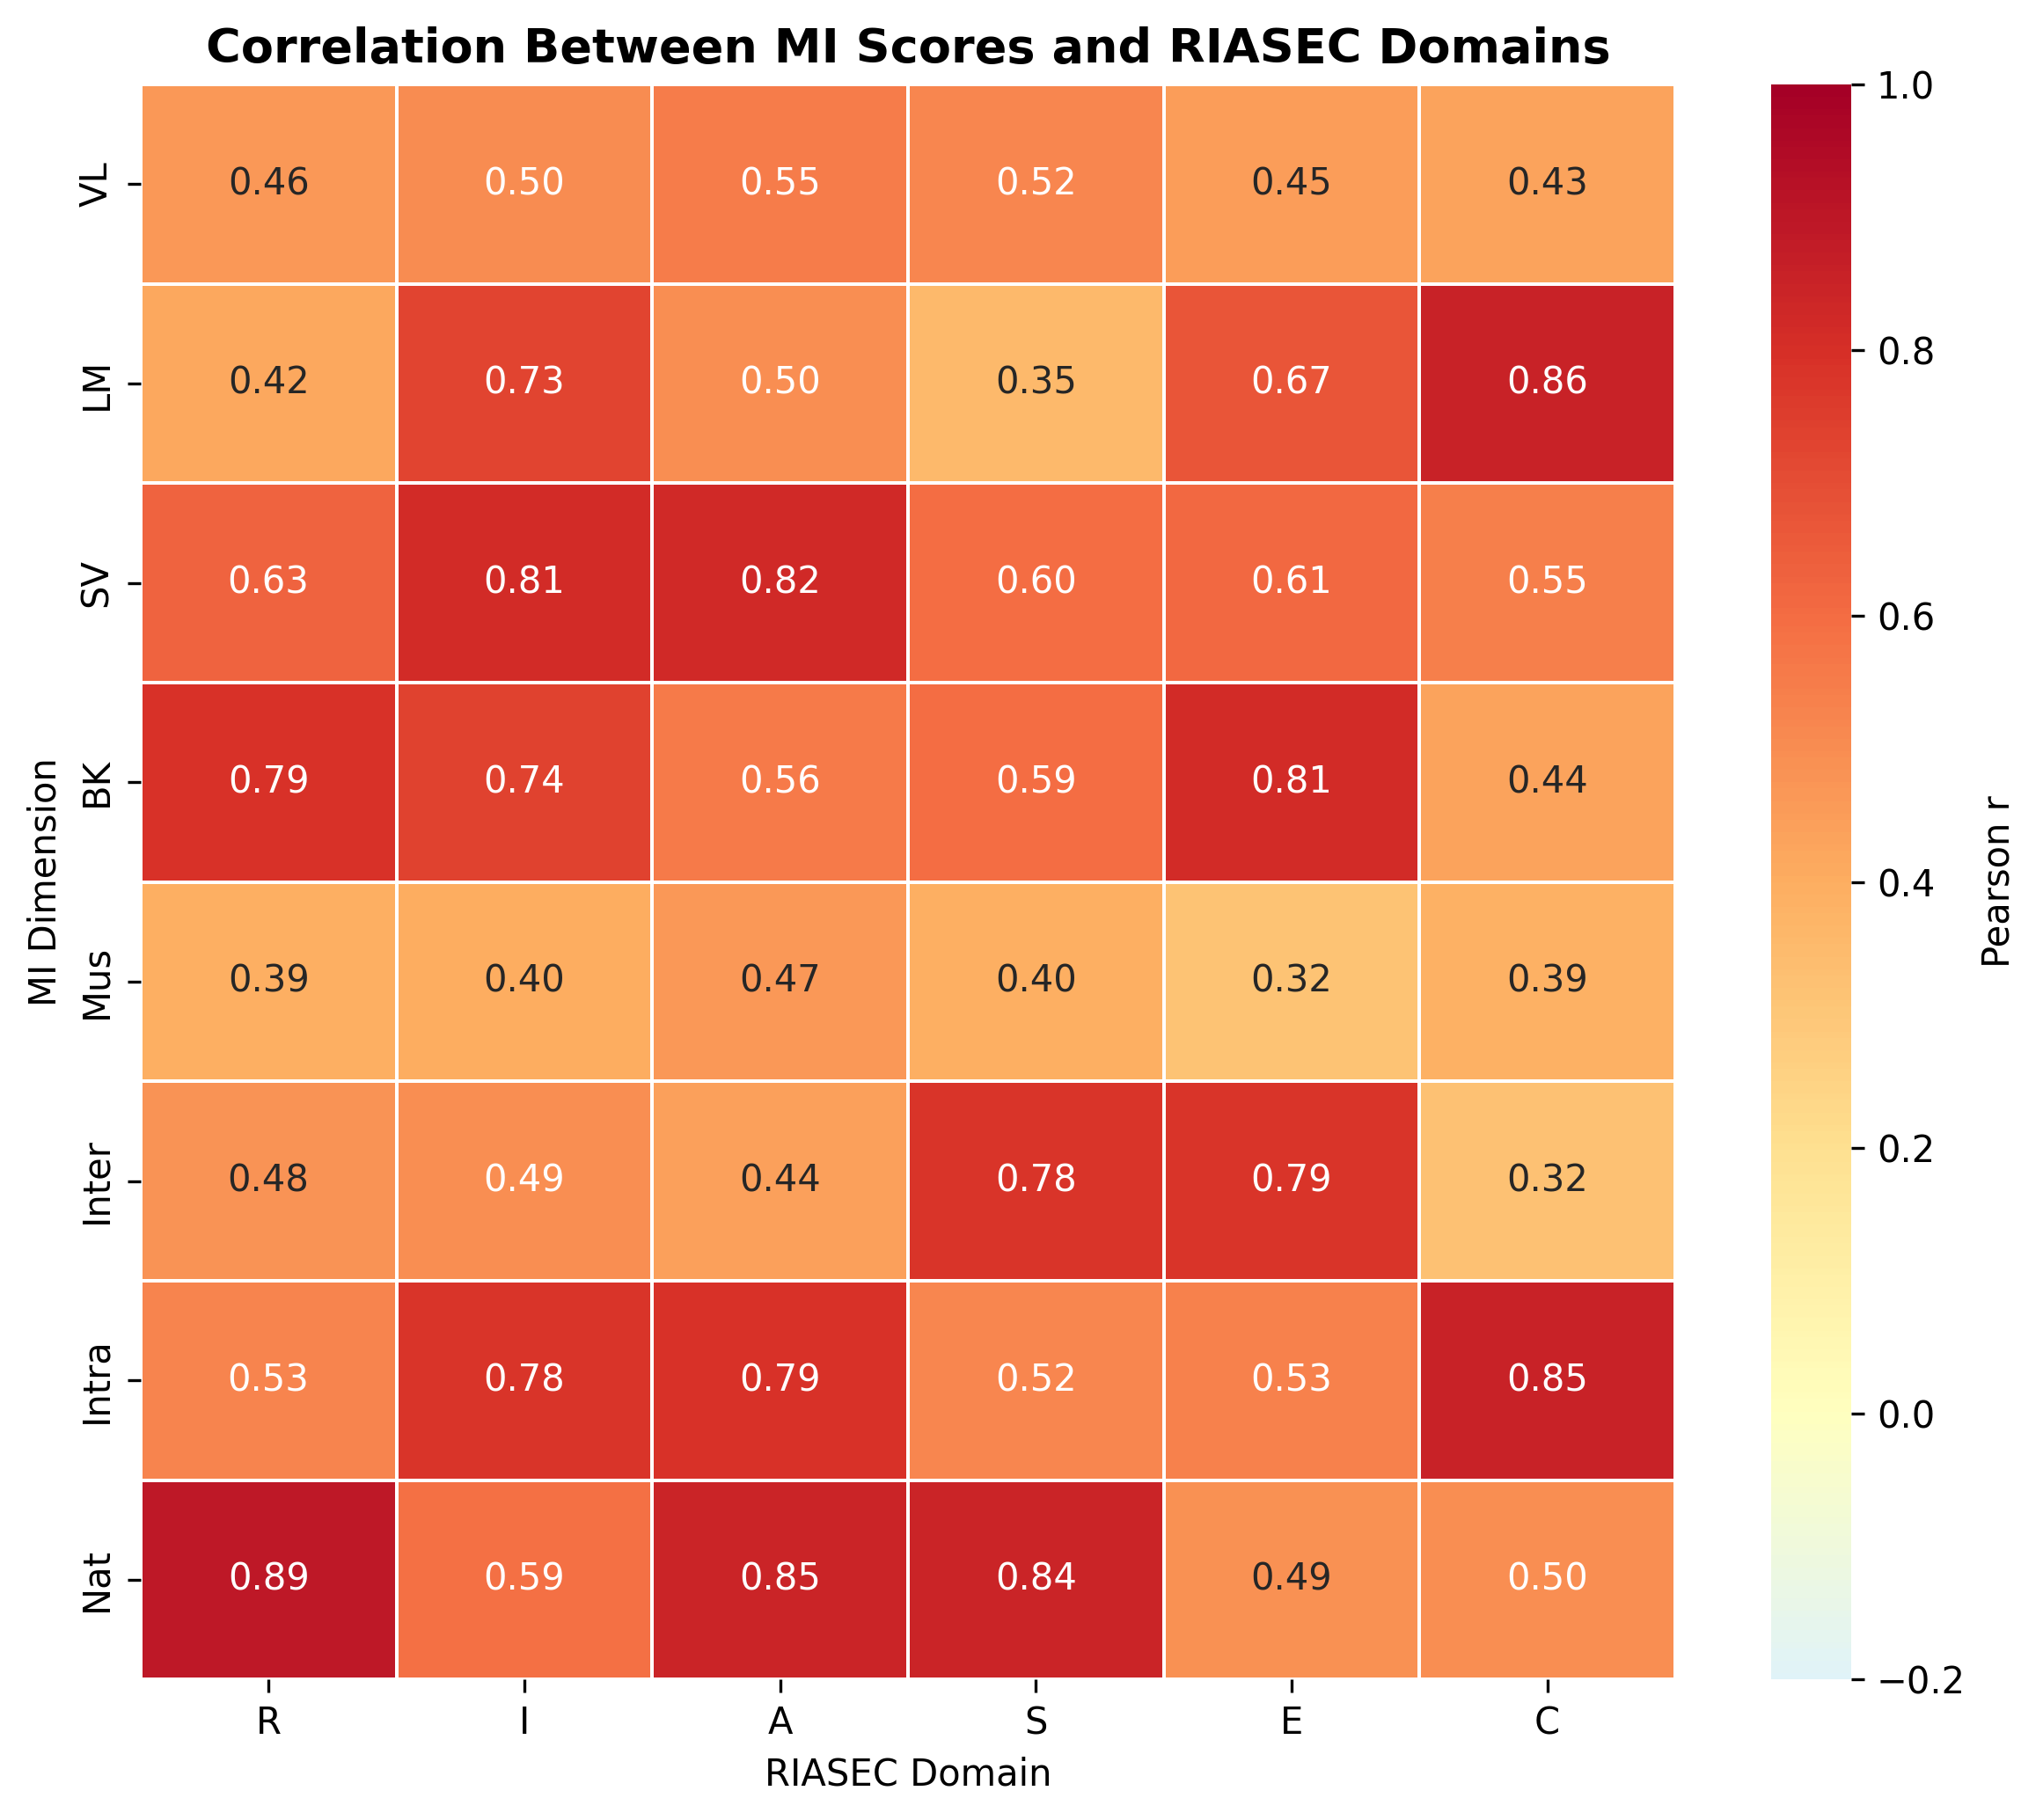
\includegraphics[width=0.85\textwidth]{../results/mi_riasec_cross_correlation.png}
    \caption{Pearson correlation matrix between MI raw scores and RIASEC domain scores. High correlations (dark red) align precisely with RIASEC formula membership (Table~\ref{tab:formula_membership}). VL and Musical dimensions, absent from all RIASEC formulas, show consistently lower correlations.}
    \label{fig:mi_riasec_corr}
\end{figure}

\subsection{Cognitive Archetypes (Unsupervised Learning)}

The Elbow method showed a significant decrease in inertia between $k=2$ and $k=3$, with diminishing returns thereafter. Silhouette scores across $k \in \{2, \ldots, 7\}$ reached a maximum at $k=2$ (0.230) and decreased monotonically, reaching 0.176 at $k=3$. While $k=2$ yields better statistical cluster cohesion, $k=3$ was selected to provide richer interpretive granularity across three distinct levels of cognitive engagement, consistent with the educational literature on differentiated instruction. The K-Means algorithm partitioned the student population into three cognitive archetypes (Silhouette Score = 0.176). PCA revealed that the first two principal components accounted for 47.5\% and 12.2\% of the total variance, respectively. The clustering results are presented in Figure~\ref{fig:clustering}. The three archetypes were distinguished primarily by their overall level of cognitive engagement: \textit{High Cognitive Engagement} ($n = 32$) showed elevated MI scores across all dimensions; \textit{Moderate Cognitive Engagement} ($n = 51$) showed mid-range scores; and \textit{Developing Cognitive Engagement} ($n = 24$) displayed lower scores across all dimensions. Figure~\ref{fig:radar} displays the radar chart of mean MI profiles per archetype, showing that profile shape is relatively consistent across clusters and that the overall engagement level---not profile orientation---is the primary differentiating dimension.

\begin{figure}[htpb]
    \centering
    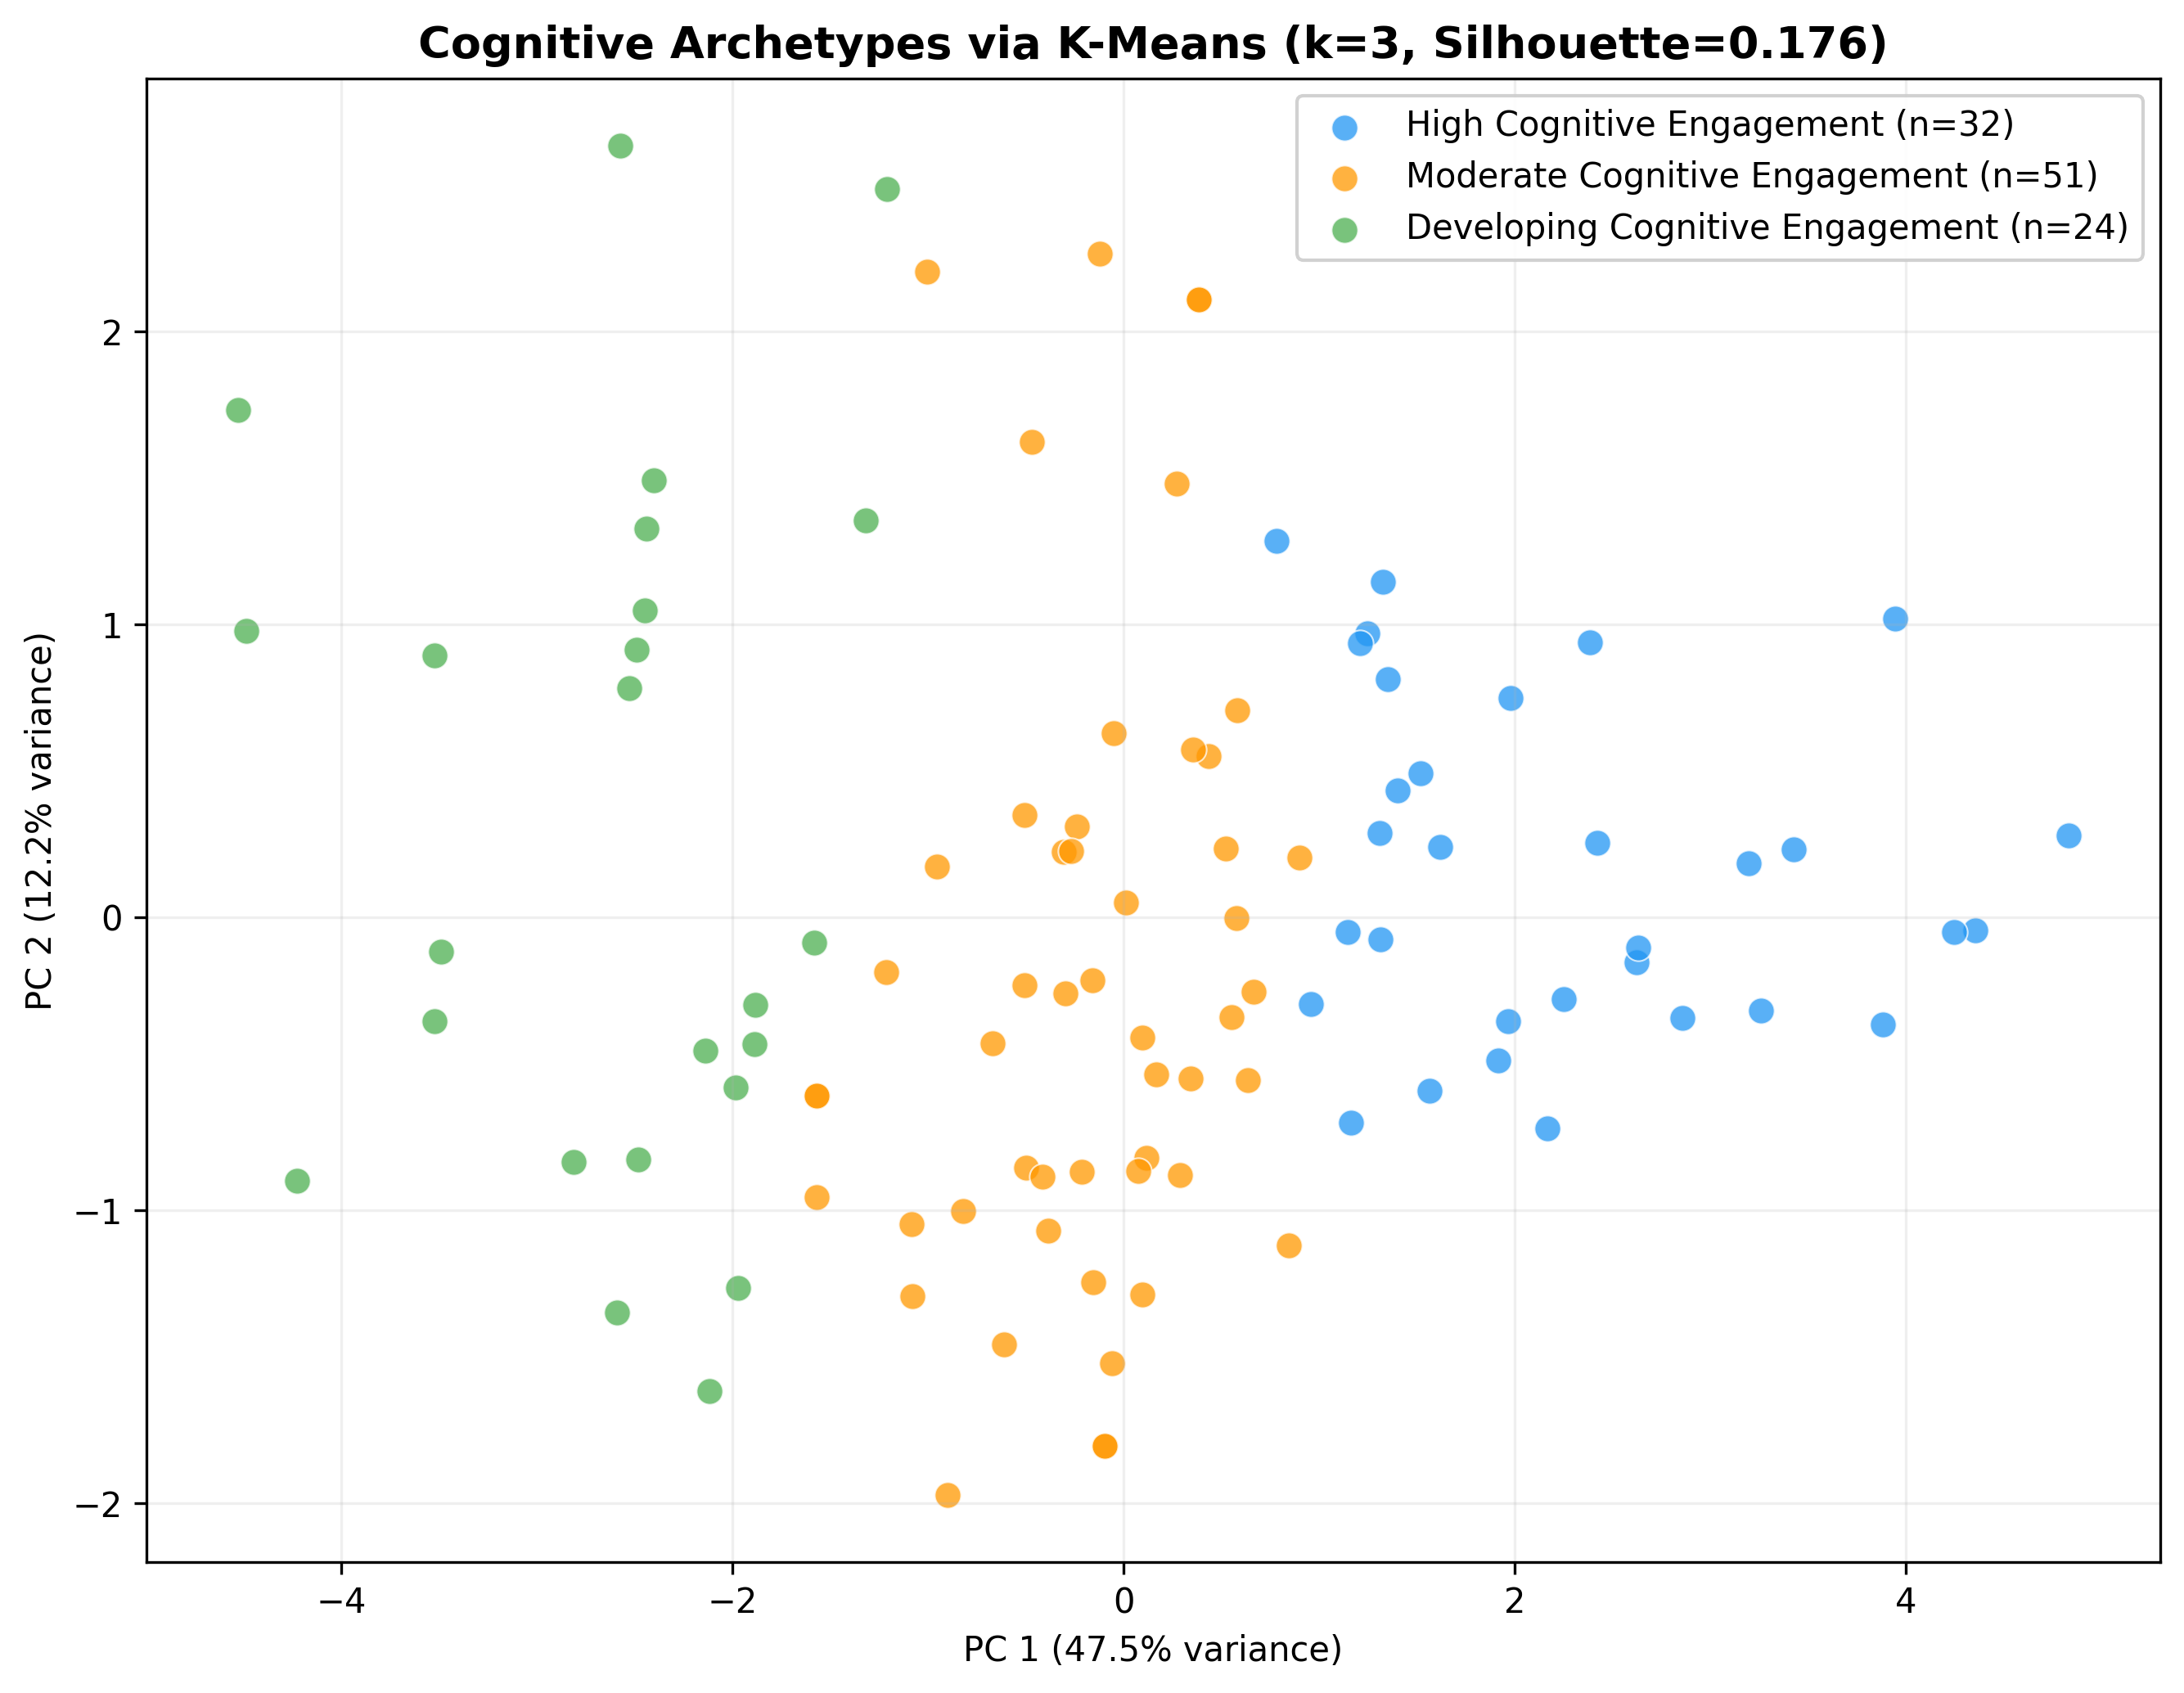
\includegraphics[width=0.85\textwidth]{../results/clustering_plot.png}
    \caption{Cognitive archetypes discovered via K-Means clustering ($k = 3$, Silhouette = 0.176) and PCA projection. Three engagement-level archetypes are identified: High ($n=32$), Moderate ($n=51$), and Developing ($n=24$).}
    \label{fig:clustering}
\end{figure}

\begin{figure}[htpb]
    \centering
    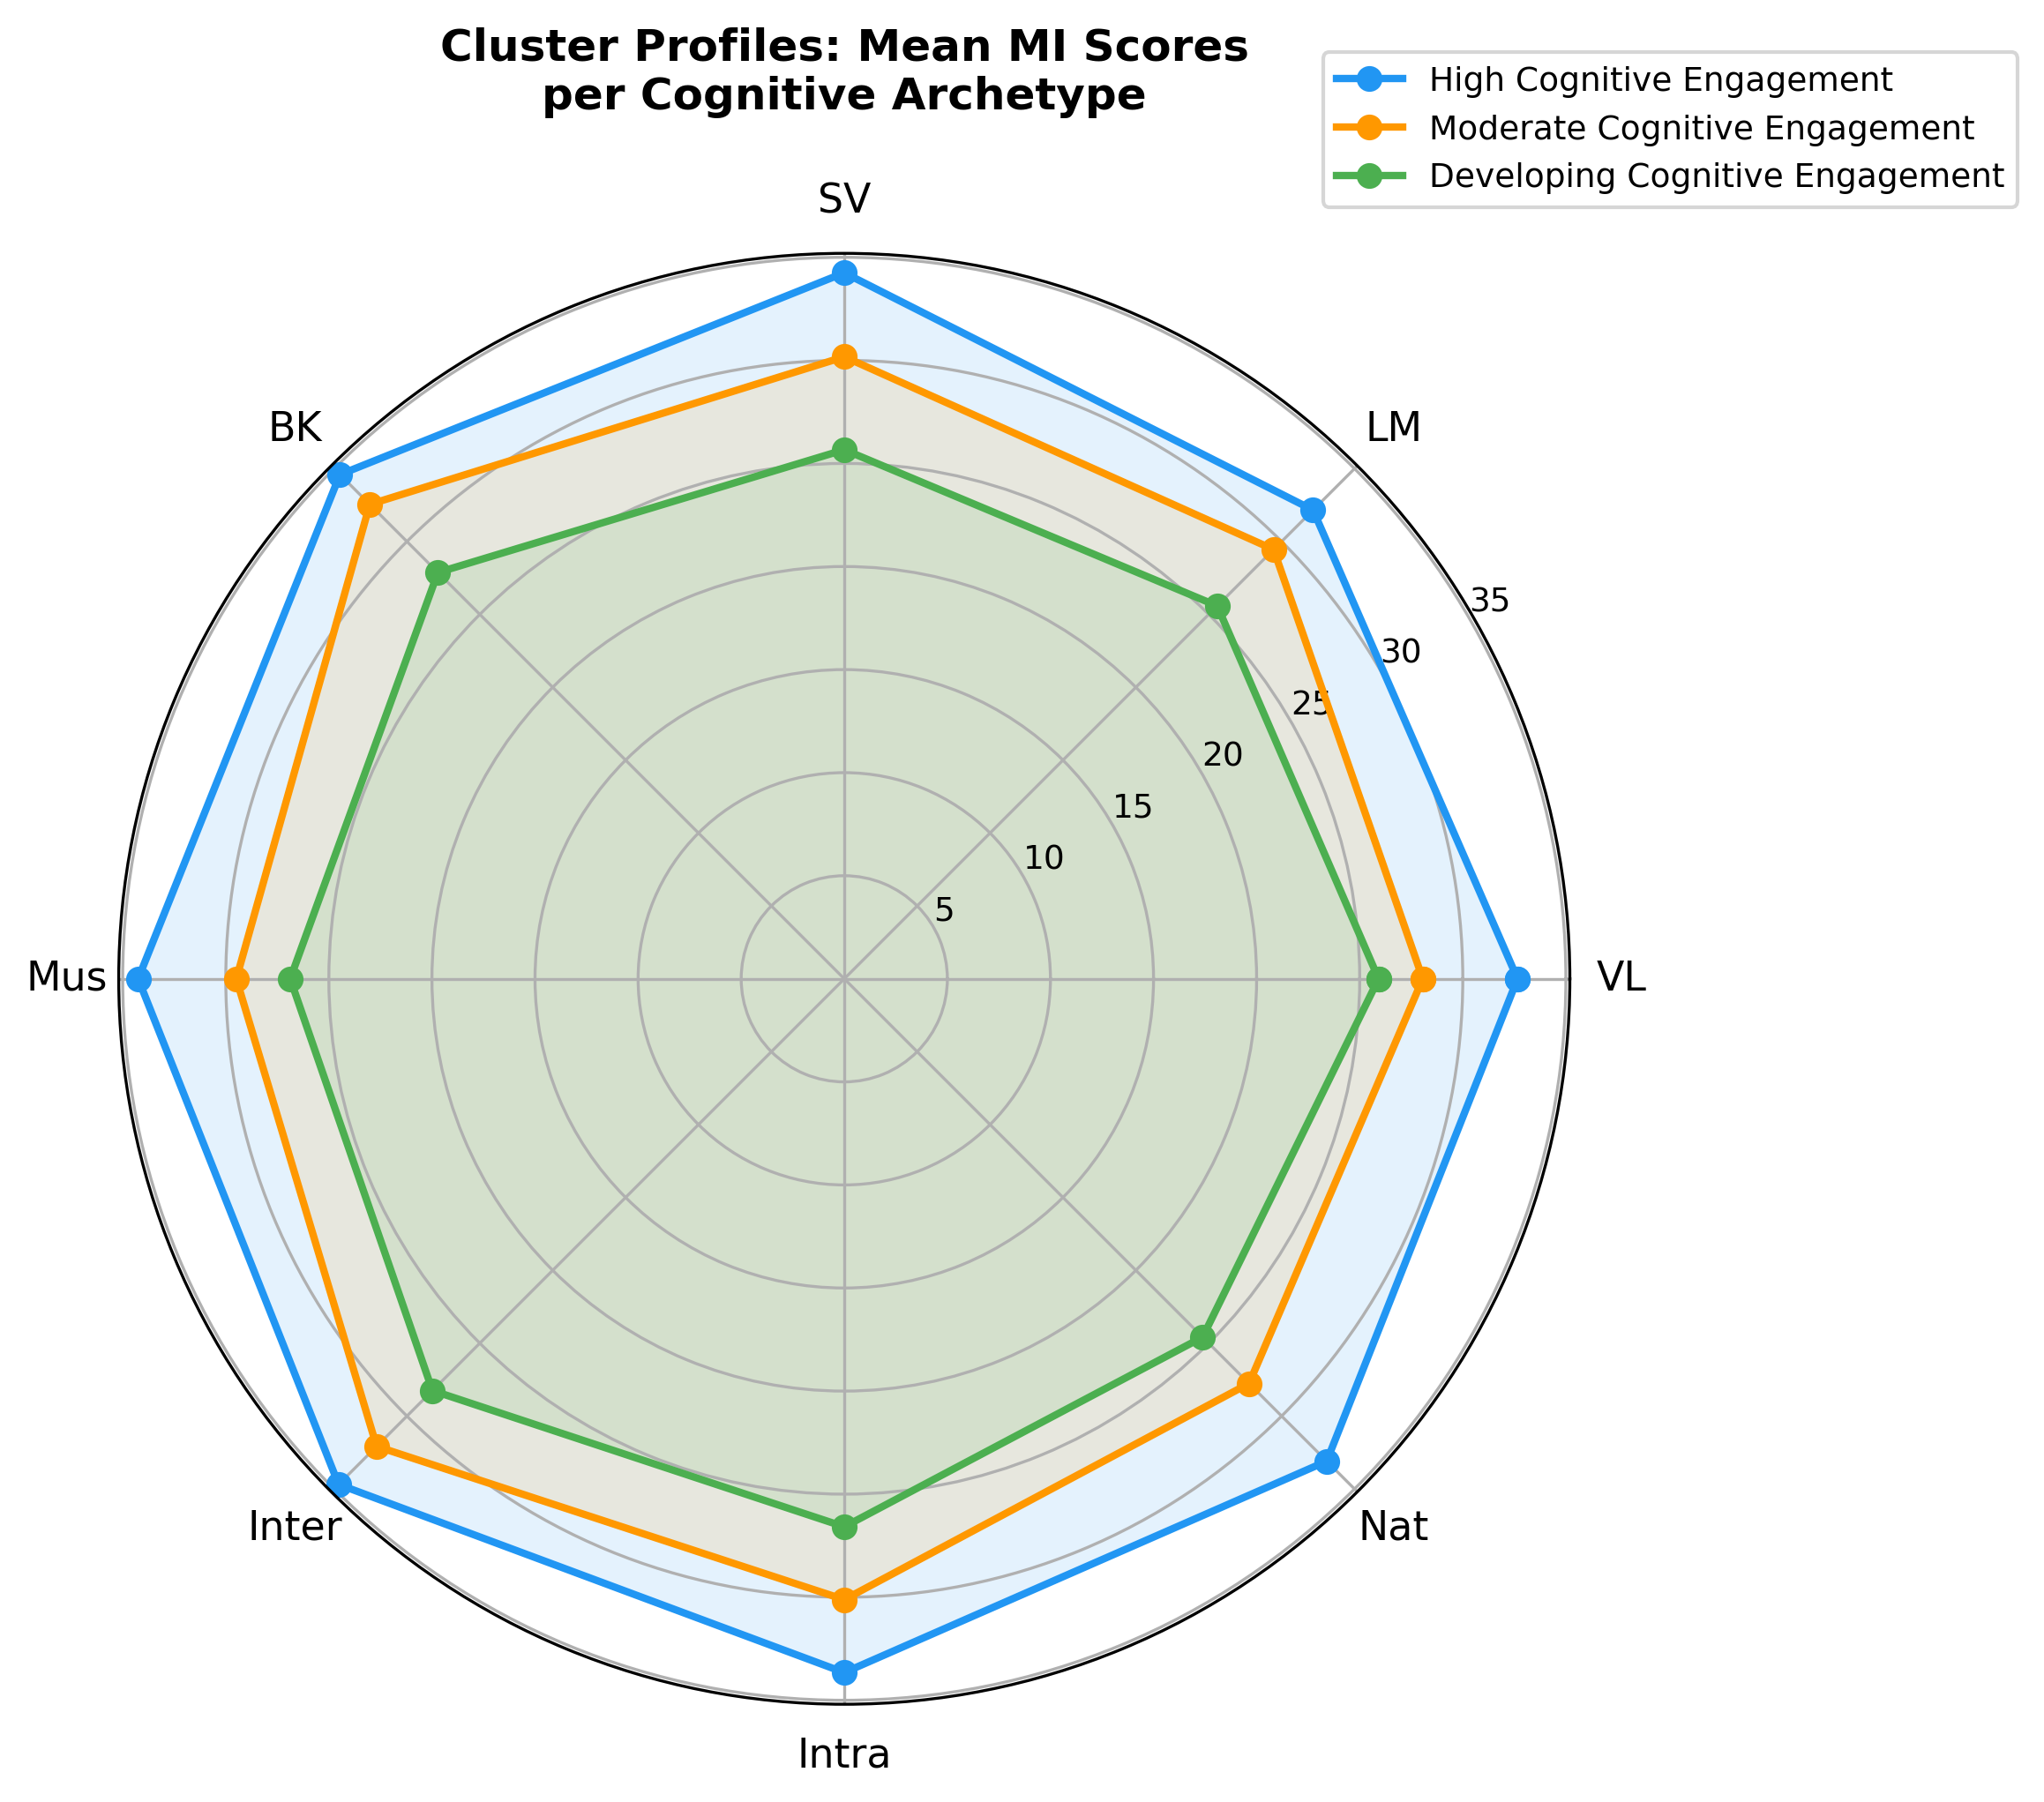
\includegraphics[width=0.78\textwidth]{../results/cluster_profiles_radar.png}
    \caption{Radar chart of mean MI raw scores per cognitive archetype. All three archetypes exhibit similar profile shape, with differences driven primarily by overall engagement level rather than relative intelligence strengths.}
    \label{fig:radar}
\end{figure}

The overall moderate Silhouette Score for clustering ($k=3$: 0.176) suggests the three-archetype solution is driven more by interpretive utility than by sharp statistical cluster boundaries. In this dataset, the Silhouette Score peaks at $k=2$ (0.230), indicating that the two-group split (overall higher vs.~lower engagement) provides the statistically cleanest partition. The $k=3$ solution was retained because it surfaces a distinguishable intermediate group (Moderate Engagement) of practical counseling relevance. These archetypes should be regarded as heuristic categories rather than discrete types, consistent with a continuous view of cognitive development. The overlapping structure in the PCA plot (Figure~\ref{fig:clustering}) reinforces this interpretation.

\subsection{Predictive Classification (Supervised Learning)}

Table~\ref{tab:model_comparison} presents the cross-validated performance of all four classifiers.

\begin{table}[htpb]
\centering
\caption{Model Comparison: Stratified 5-Fold Cross-Validation Results ($N = 107$, 6 classes)}
\label{tab:model_comparison}
\small
\begin{tabular}{lcc}
\toprule
Model & Accuracy ($M \pm SD$) & F1-Weighted ($M \pm SD$) \\
\midrule
Logistic Regression    & $\mathbf{0.815 \pm 0.090}$ & $\mathbf{0.791 \pm 0.094}$ \\
Gradient Boosting      & $0.628 \pm 0.094$ & $0.578 \pm 0.092$ \\
SVM (RBF Kernel)       & $0.618 \pm 0.075$ & $0.530 \pm 0.070$ \\
Random Forest          & $0.562 \pm 0.087$ & $0.508 \pm 0.068$ \\
\midrule
Majority-Class Baseline & $0.308$ & --- \\
Random Baseline        & $0.167$ & --- \\
\bottomrule
\end{tabular}
\end{table}

Logistic regression achieved the highest cross-validated accuracy of 81.5\% ($M \pm SD = 0.815 \pm 0.090$), substantially outperforming all other models, the majority-class baseline of 30.8\% (always predicting Enterprising), and the equal-probability random baseline of 16.7\%. A one-sample $t$-test comparing LR fold accuracies against the random baseline confirmed statistical significance ($t(4) = 14.48$, $p < .001$, 95\%~CI [0.691, 0.939]). This finding suggests that the relationship between MI scores and dominant RIASEC domain is predominantly linear, which is theoretically coherent: each RIASEC score is itself a linear function of a MI subset (Equations 4--5), making linear separability structurally inherent to the classification task. Non-linear models (Random Forest, Gradient Boosting, SVM) yielded lower accuracy, likely due to overfitting given the small dataset ($N = 107$).

Figure~\ref{fig:confusion} presents the confusion matrices for the Logistic Regression model (best performer) on both the hold-out test set and cross-validated predictions.

\begin{figure}[htpb]
    \centering
    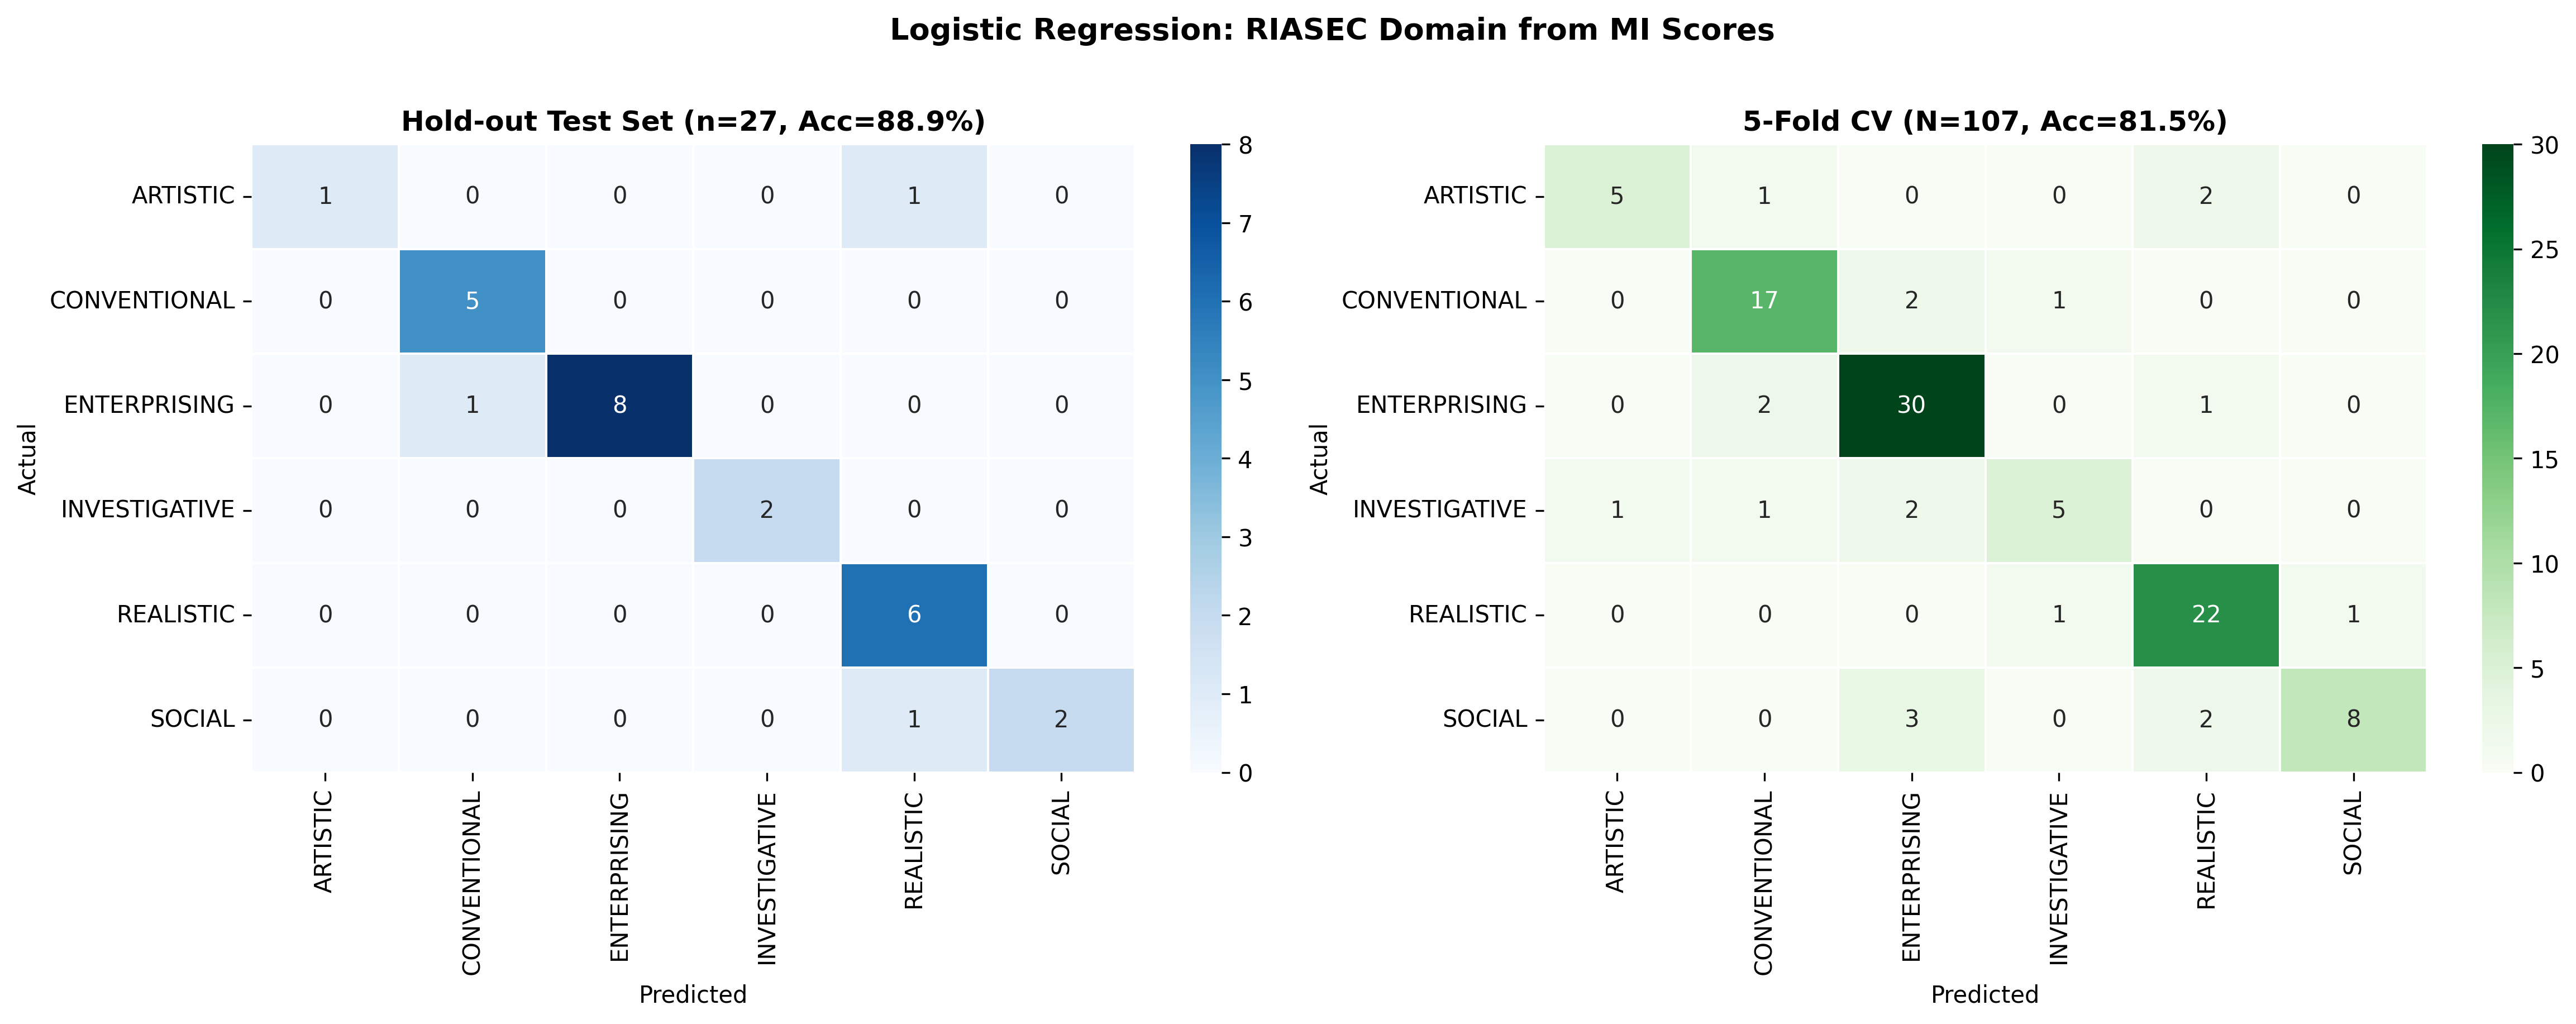
\includegraphics[width=\textwidth]{../results/confusion_matrix.png}
    \caption{Confusion matrices for Logistic Regression (best model): hold-out test set (left; $n = 27$, Acc = 88.9\%) and 5-fold cross-validation (right; $N = 107$, Acc = 81.5\%).}
    \label{fig:confusion}
\end{figure}

Figure~\ref{fig:model_comparison} visualizes the comparative performance across all four classifiers.

\begin{figure}[htpb]
    \centering
    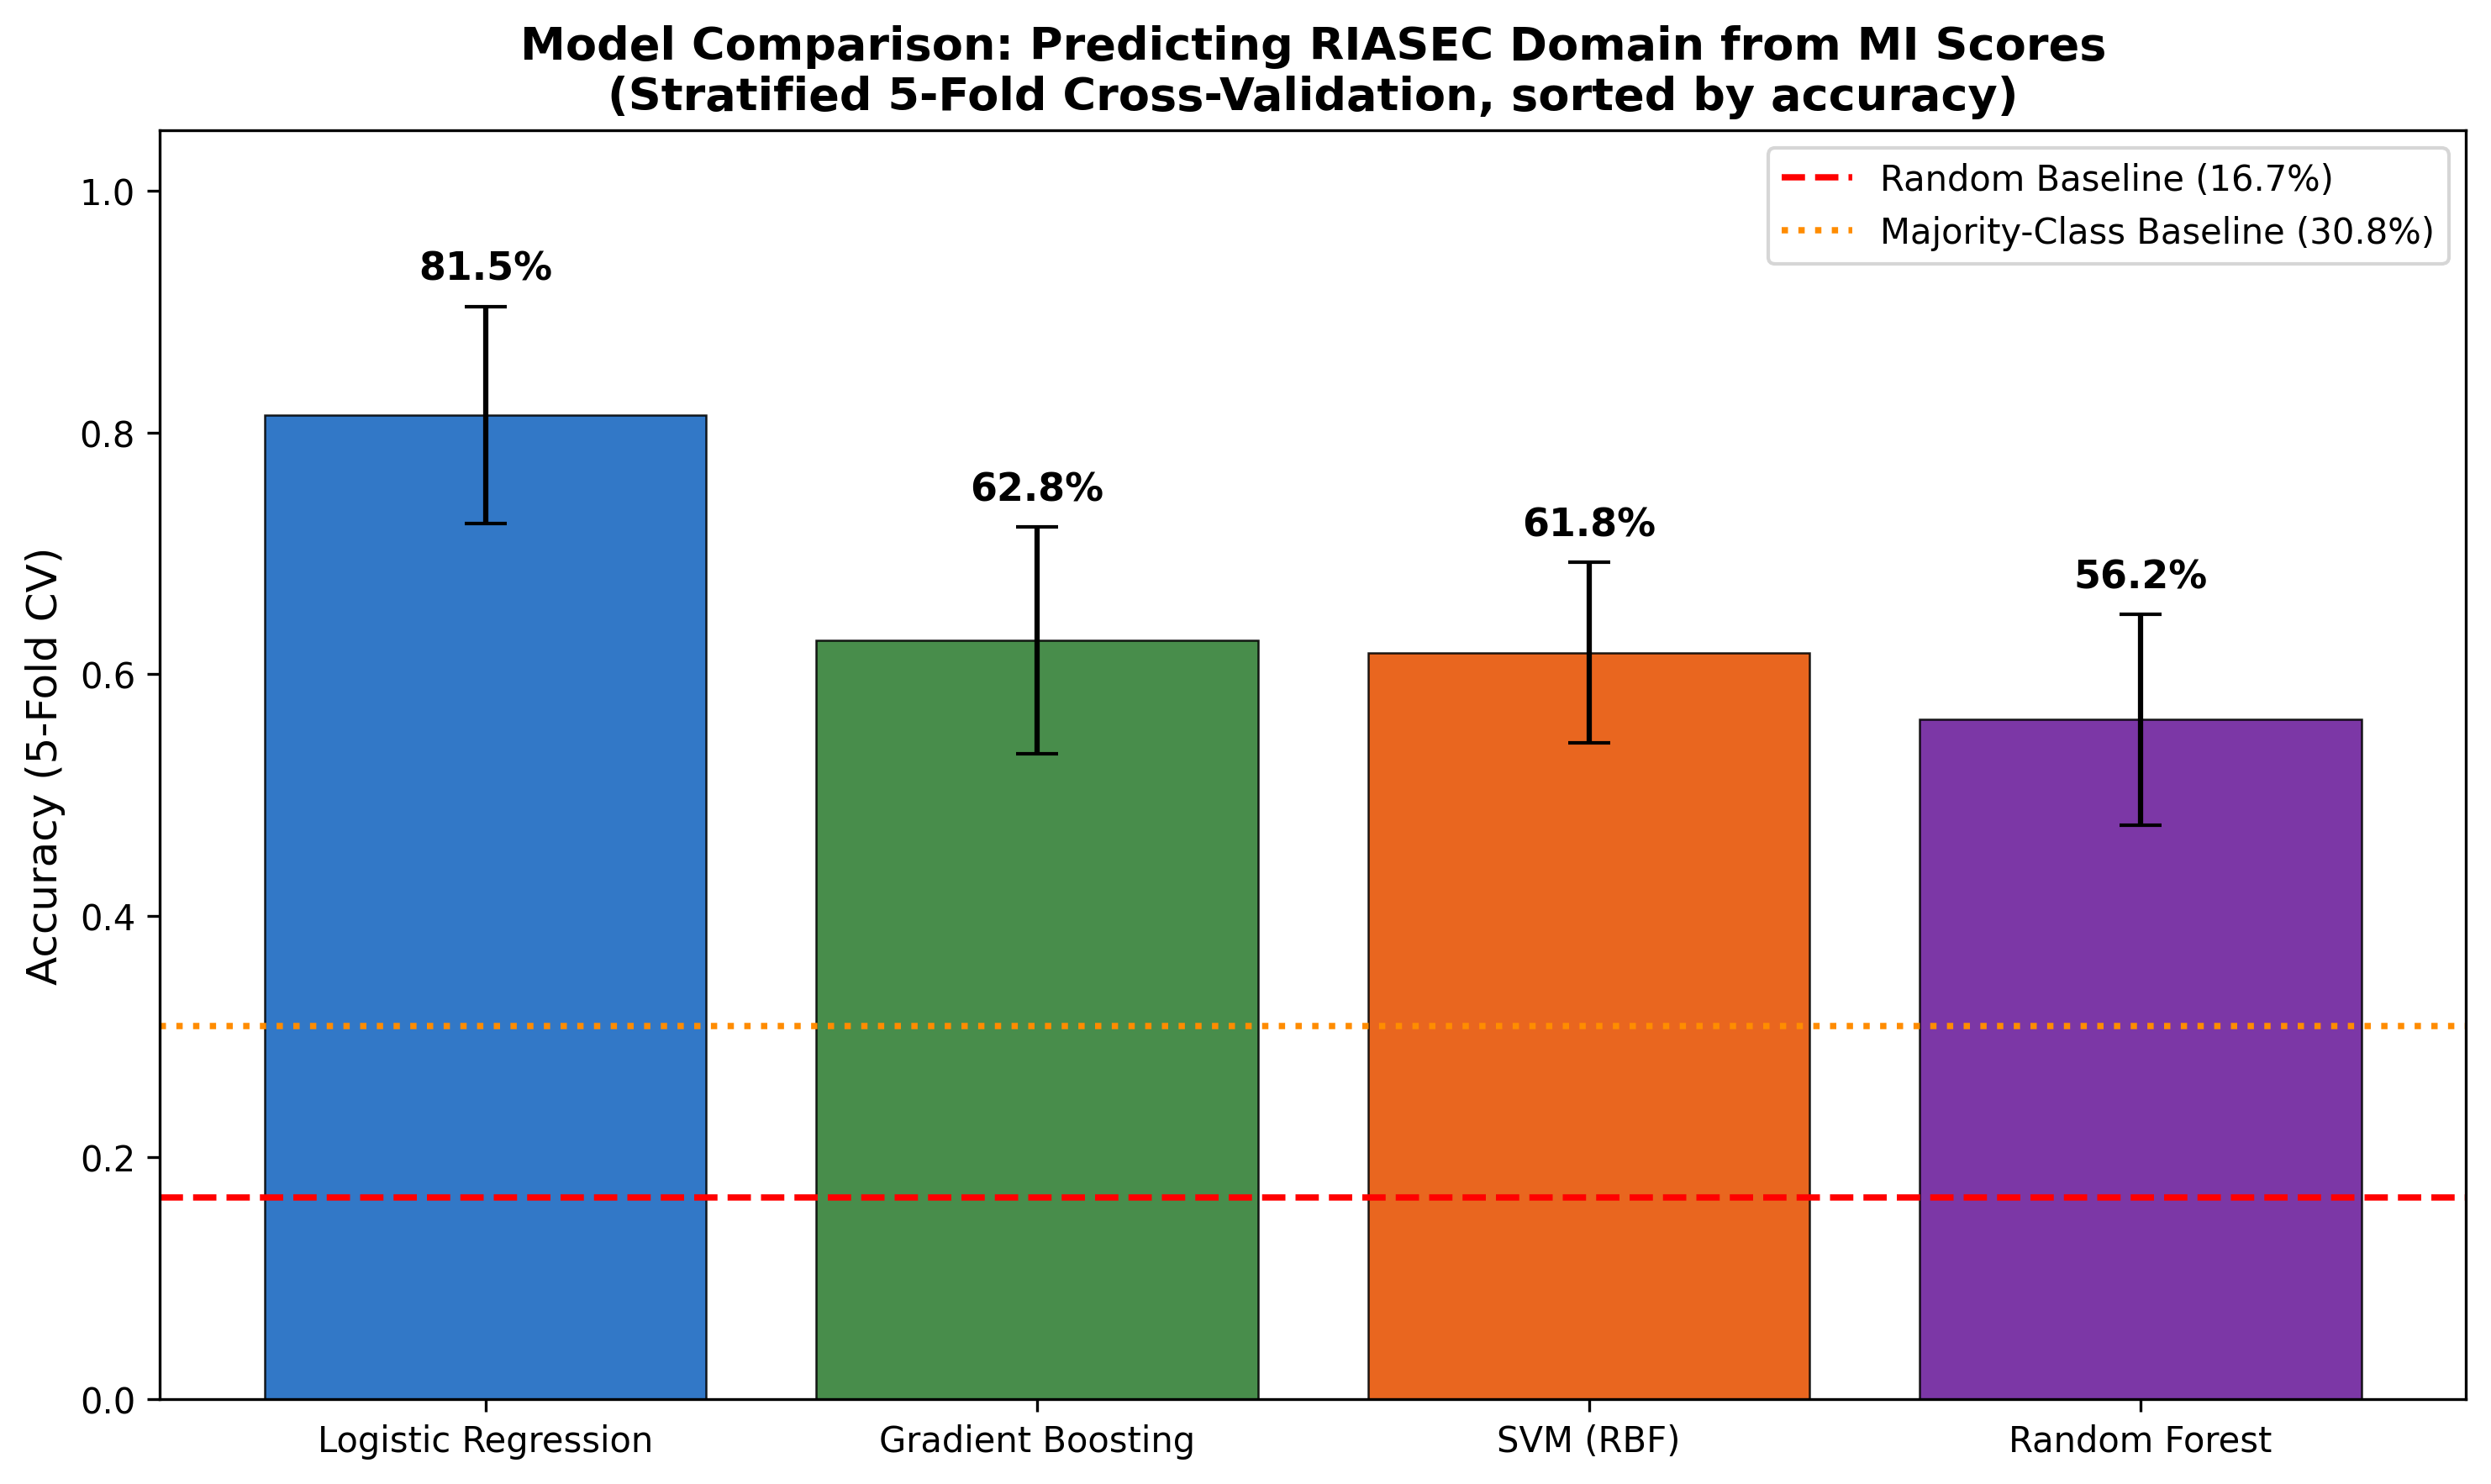
\includegraphics[width=0.8\textwidth]{../results/model_comparison.png}
    \caption{Comparison of classifier accuracy (5-fold stratified CV, sorted by accuracy). Dashed red line: equal-probability random baseline (16.7\%). Dotted orange line: majority-class baseline (30.8\%).}
    \label{fig:model_comparison}
\end{figure}

\subsection{Model Transparency via SHAP}

To identify which MI dimensions most strongly influence RIASEC domain predictions, SHAP analysis was performed on the Random Forest model, selected for its tree-based architecture which supports the exact \texttt{TreeExplainer} algorithm. The SHAP feature importance summary decomposed by RIASEC class is shown in Figure~\ref{fig:shap}. The most influential feature overall was Naturalist with a mean $|$SHAP$| \approx 0.41$, followed by Bodily-Kinesthetic (0.22) and Interpersonal (0.20). Theoretically, Naturalist intelligence contributes to three RIASEC formulas (R, A, S) while being absent from the remaining three (I, E, C), creating a strong discriminative signal. Bodily-Kinesthetic features in three formulas (R, I, E) and Interpersonal in two (S, E), which accounts for their secondary importance. Notably, Verbal-Linguistic and Musical intelligences---which contribute to no RIASEC formula---nonetheless exhibit small non-zero SHAP values, reflecting non-linear correlational patterns captured by the Random Forest that transcend the linear formula structure.

\begin{figure}[htpb]
    \centering
    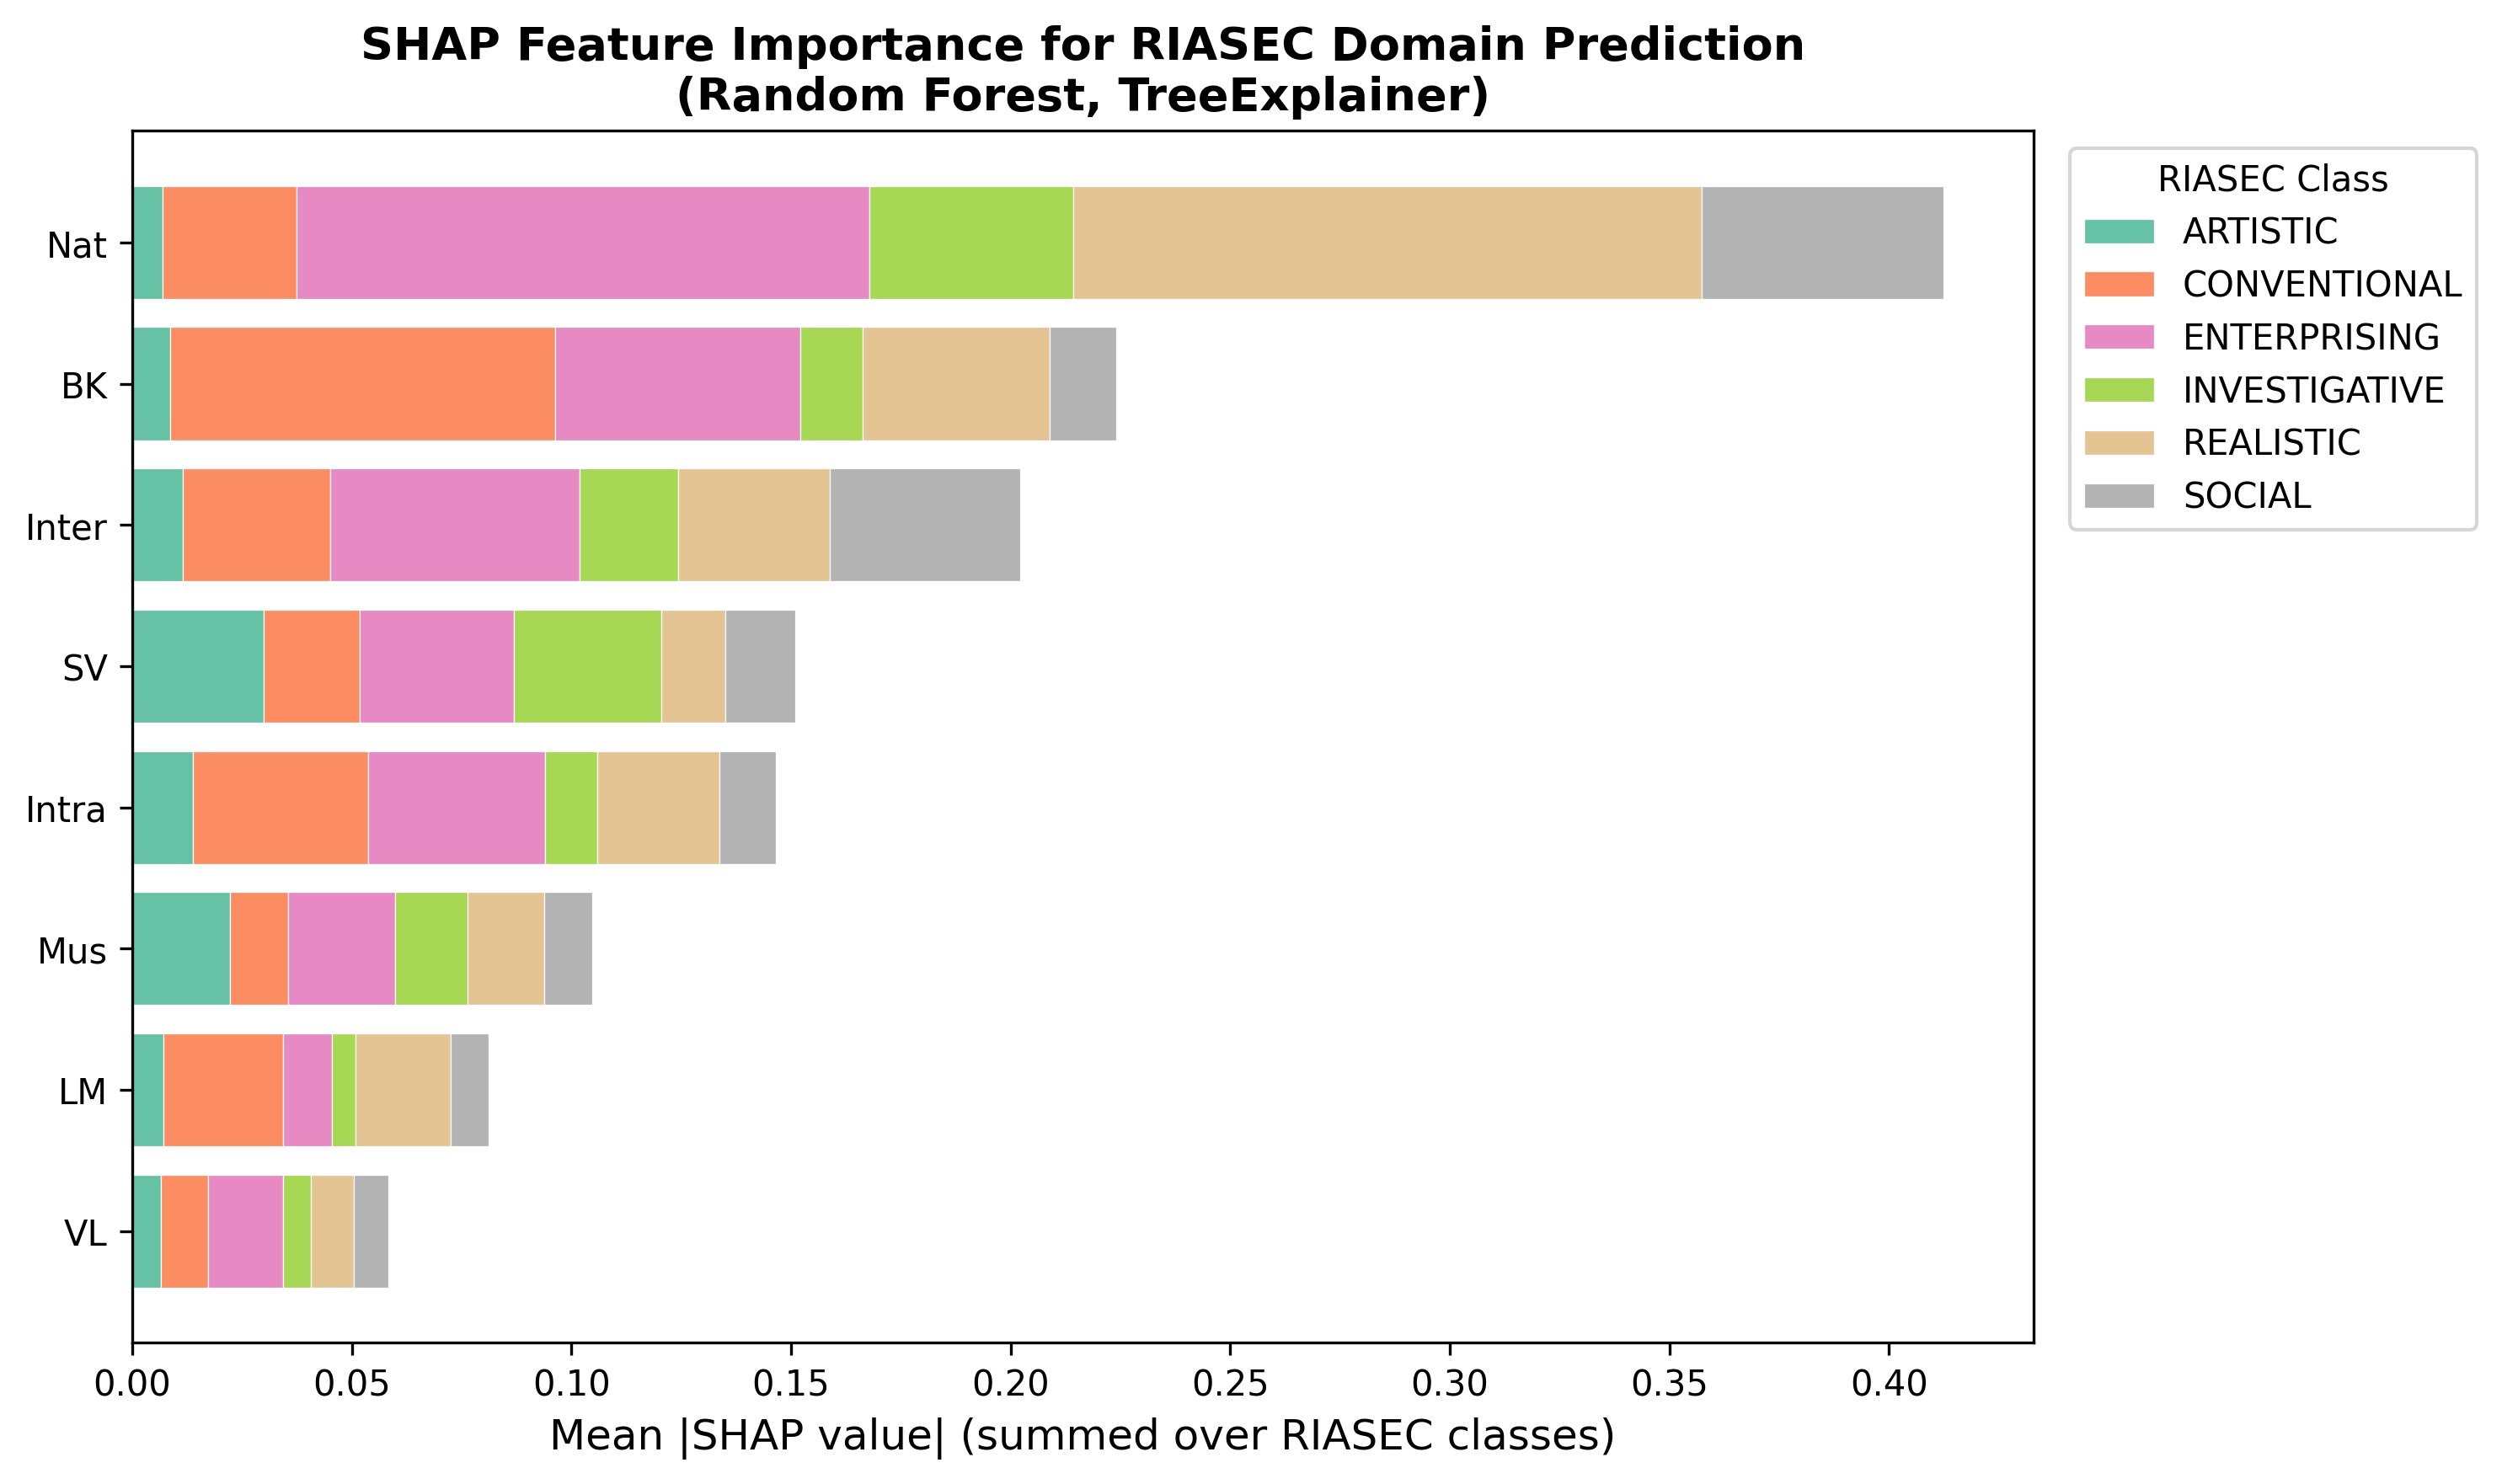
\includegraphics[width=0.85\textwidth]{../results/shap_summary.png}
    \caption{SHAP feature importance summary, decomposed by RIASEC class contributions.}
    \label{fig:shap}
\end{figure}

\section{Discussion}

The results of this study provide an empirical basis for the effectiveness of machine learning in bridging cognitive profiling (MI) and vocational mapping (RIASEC). Logistic regression's 81.5\% cross-validated accuracy demonstrates that eight MI scores contain sufficient information to reliably predict a student's dominant vocational orientation.

\subsection{Theoretical Implications}

One notable and theoretically coherent result is the dominance of linear logistic regression over ensemble methods. Because each RIASEC score is a linear function of a MI subset (Equations 4--5), predicting the \textit{dominant} RIASEC domain from raw MI inputs involves identifying which of six overlapping linear combinations achieves the maximum value---a task with inherently linear separability. The more flexible ensemble methods (Random Forest, Gradient Boosting) and SVM offered no advantage because the underlying generative structure is already linear, and with $N = 107$ and $p = 8$ features, their additional parameters introduce overfitting. This result is consistent with \citeauthor{guleria2022explainable}'s \citeyear{guleria2022explainable} recommendation that simpler, interpretable models should be preferred in educational AI contexts when accuracy is competitive.

The SHAP analysis showed that Naturalist intelligence is the single most discriminative MI dimension for vocational prediction. This discriminative power arises from its \textit{selective} presence: it appears in Realistic, Artistic, and Social formulas while being absent from Investigative, Enterprising, and Conventional---creating a structural partition between two broad clusters of RIASEC domains (RAS vs.\ IEC). Bodily-Kinesthetic and Interpersonal intelligences similarly derive their predictive utility from selective formula membership. Notably, Verbal-Linguistic and Musical intelligences---absent from all RIASEC formulas---exhibit small non-zero SHAP values (0.06 and 0.10 respectively), indicating that their residual correlational patterns are detected by the Random Forest beyond the linear formula structure; this finding invites further investigation into the indirect role these intelligences may play in vocational inclination.

A deeper theoretical implication follows: because the Investigative domain uniquely incorporates four MI dimensions (Bodily-Kinesthetic, Intrapersonal, Logical-Mathematical, and Spatial-Visual), the common stereotype equating investigative careers exclusively with ``logical'' intelligence is empirically refined. The instrument operationalizes Investigative vocational inclination as a more embodied and spatially engaged cognitive profile, incorporating physical coordination (BK) and self-awareness (Intra) alongside analytical reasoning (LM) and spatial visualization (SV).

\subsection{Practical Implications}

The automated extraction and prediction pipeline developed in this study offers a scalable approach to career counselling. By transforming subjective questionnaire responses into structured, machine-interpretable feature vectors, counsellors can receive data-driven recommendations that complement their professional judgment \cite{kamal2021smart}. The integration of XAI ensures that these recommendations are transparent and auditable, addressing concerns about algorithmic bias and opacity in educational settings \cite{zhang2022integrating, crompton2023artificial}.

A key pedagogical insight of the clustering analysis---identifying the High, Moderate, and Developing Cognitive Engagement archetypes---is that students vary more in their overall level of cognitive engagement than in the shape of their profile. This suggests that general interventions aimed at increasing academic motivation may be more effective than those targeting specific intelligences. Counsellors may use these archetypes as an initial triage, adjusting the depth of vocational advisory support to each student's cognitive engagement profile.

\subsection{Limitations}

Several limitations must be acknowledged. \textit{First}, the sample size ($N = 107$) is relatively small for a six-class classification problem, potentially limiting the generalisability of results and constraining the performance of ensemble methods. \textit{Second}, the sample is drawn from a single institution in one geographic region (Mumbai, India); cultural variation in MI self-reporting \cite{shearer2018multiple} and differences in Indian secondary-school vocational aspirations may limit cross-cultural applicability. \textit{Third}---and most critically---the dominant RIASEC class is a deterministic linear function of the same MI raw scores used as features. This structural circularity means that the reported 81.5\% accuracy reflects, in part, the model's recovery of the scoring formula rather than genuine predictive validity against independently observed career outcomes. Future work must validate these models using independently administered RIASEC assessments (e.g., Holland's Self-Directed Search \citeyear{holland1997making}) to establish convergent validity and rule out artifactual inflation. \textit{Fourth}, the 80-item self-report questionnaire is subject to social-desirability bias, response-set effects, and the general limitations of Likert-scale self-report \cite{sackett2017individualized}. \textit{Fifth}, the psychometric properties of the commercially administered instrument (e.g., internal consistency via Cronbach's $\alpha$, test-retest reliability) were not independently assessed; the authors relied on the instrument provider's reported standardization. \textit{Sixth}, the $t$-test on five-fold accuracy estimates uses only $df = 4$ and assumes independence of folds, which is an approximation; a permutation test on the full dataset would provide a more robust significance estimate.

\section{Conclusion}

This study demonstrates that machine learning can effectively map Multiple Intelligence profiles to RIASEC vocational domains, achieving 81.5\% cross-validated accuracy (88.9\% hold-out, $n = 27$) using logistic regression---a nearly five-fold improvement over the equal-probability random baseline of 16.7\% and more than 2.6-fold improvement over the majority-class baseline of 30.8\% ($t(4) = 14.48$, $p < .001$). The empirical verification of all six RIASEC scoring formulae---including the novel finding that the Investigative domain draws upon four MI dimensions (Bodily-Kinesthetic, Intrapersonal, Logical-Mathematical, and Spatial-Visual)---contributes a more granular theoretical understanding of the MI--RIASEC relationship than previously documented. By combining unsupervised clustering for cognitive engagement archetype discovery, supervised multi-class classification for vocational domain prediction, and SHAP-based explainable AI for transparent feature attribution, this study contributes a replicable, end-to-end framework for data-driven career counselling.

The transparent formula structure---where specific MI dimensions map deterministically to RIASEC subsets---provides counsellors with a principled and auditable basis for explaining psychometric outputs to students and parents. The Pearson correlations between MI and RIASEC scores (up to $r = .89$ for Naturalist--Realistic) provide independent psychometric evidence of the structural validity of this mapping.

Future research should: (1) extend this framework to larger, multi-institutional, and geographically diverse datasets; (2) validate ML-predicted RIASEC domains against independently administered vocational assessments to address the structural circularity identified herein; and (3) employ longitudinal designs to examine whether MI-to-RIASEC predictions at the secondary school stage translate to improved career satisfaction and stability in adulthood.

The complete anonymized dataset and reproducible analysis code are publicly available at: \url{https://github.com/sunny-nanade/mi-riasec-ml}.

\section{AI Use Statement}

In the preparation of this manuscript, AI tools were utilized for data extraction automation, statistical verification, and initial document structuring. The authors have rigorously reviewed, verified, and validated all data, code, analyses, and text, taking full responsibility for the accuracy and integrity of the content.

\section{CRediT Author Statement}

\textbf{Sanket Gudekar}: Conceptualization, Data curation, Formal analysis, Software, Writing---Original draft. \textbf{Sunny Nanade}: Supervision, Methodology, Validation, Resources, Writing---Review \& Editing.

\bibliographystyle{apacite}
\bibliography{references}

\end{document}
